% Presentation.tex
% ================================================================
% Presentación Técnica del Plan de Mantenimiento - Yoliztli
% Versión: Oscura (Azul Premium/Técnico), Texto Grande y Minimalista
% Compilar con: lualatex Presentation.tex
% Aspect Ratio: 16:9 (Moderno)
% ================================================================

\documentclass[aspectratio=169, 12pt]{beamer}

% --- Idioma y Fuentes ---
\usepackage[spanish,es-tabla]{babel}
\usepackage{fontspec}
\usepackage{csquotes}

% --- Diseño y Gráficos ---
\usepackage{graphicx}
\usepackage{tikz}
\usetikzlibrary{positioning, shapes.geometric, arrows.meta, fit, backgrounds, calc}
\usepackage{booktabs}
\usepackage{tabularx}

% --- Configuración Estética Minimalista ---
\usetheme{default}
\usecolortheme{default}
\usefonttheme{professionalfonts}

% Desactivar barra de navegación de Beamer
\setbeamertemplate{navigation symbols}{}
\setbeamertemplate{headline}{}

% Colores del proyecto (Paleta Oscura Azul Premium)
\definecolor{darkbg}{RGB}{10, 16, 26}        % Azul marino profundo
\definecolor{cardbg}{RGB}{18, 28, 45}        % Azul pizarra para contenedores
\definecolor{lighttext}{RGB}{220, 230, 242}  % Texto claro (azul-blanco)
\definecolor{techblue}{RGB}{64, 156, 255}    % Azul eléctrico principal
\definecolor{accentcyan}{RGB}{0, 210, 255}   % Cian brillante para acentos
\definecolor{accentgreen}{RGB}{50, 220, 120} % Verde éxito
\definecolor{accentred}{RGB}{255, 80, 80}    % Rojo coral
\definecolor{accentorange}{RGB}{255, 165, 0} % Naranja vibrante
\definecolor{white}{RGB}{255, 255, 255}

\setbeamercolor{background canvas}{bg=darkbg}
\setbeamercolor{normal text}{fg=lighttext}
\setbeamercolor{title}{fg=techblue}
\setbeamercolor{frametitle}{fg=techblue}
\setbeamercolor{structure}{fg=techblue}

% Formato de bloques en tema oscuro
\setbeamercolor{block title}{bg=cardbg,fg=techblue}
\setbeamercolor{block body}{bg=cardbg,fg=lighttext}

% Formato de listas (bullets minimalistas)
\setbeamertemplate{itemize items}[circle]

% Diseño del título del frame (Frametitle MÁS GRANDE)
\setbeamertemplate{frametitle}{
    \vspace{0.4cm}
    \begin{minipage}{\textwidth}
        {\LARGE\bfseries\color{techblue}\insertframetitle}
        \par\vspace{0.15cm}
        {\color{techblue!40}\hrule height 1.5pt}
    \end{minipage}
}

% Diseño del pie de página (Footline) - Solo números de página
\setbeamertemplate{footline}{
    \begin{beamercolorbox}[wd=\paperwidth,ht=0.8cm,dp=0.4cm,right]{footline}
        \color{lighttext!40}\footnotesize
        \insertframenumber\ / \inserttotalframenumber\hspace{0.8cm}
    \end{beamercolorbox}
}

% Comandos personalizados
\newcommand{\statusdot}[1]{\tikz\draw[#1,fill=#1] (0,0) circle (0.5ex);}

% --- Información de la Presentación ---
\title{PLAN DE MANTENIMIENTO DE SOFTWARE}
\subtitle{Proyecto Yoliztli --- Sistema Educativo Infantil}
\author[Equipo de Mantenimiento]{
    Brandon Chavarría Ángeles \and
    Emmanuel Islas Lozada \and
    Kenneth Morán Gómez \and
    José Enrique Sánchez Romero
}
\institute[UPP]{
    Ingeniería en Software --- Mantenimiento de Software \\
    Universidad Politécnica de Pachuca
}
\date{\today}

% ================================================================
\begin{document}

% Slide 1: Portada (Estética Oscura Minimalista con Logo Ajustado en la Esquina)
\begin{frame}[plain]
    \begin{tikzpicture}[remember picture,overlay]
        % Decoración de fondo abstracta
        \begin{scope}[opacity=0.03]
            \draw[techblue, line width=1.5pt] (current page.south west) ++(2,0) -- +(45:12);
            \draw[techblue, line width=2pt] (current page.south west) ++(4,0) -- +(35:15);
            \draw[techblue, line width=1.5pt] (current page.south east) circle (4cm);
            \draw[techblue, line width=1pt] (current page.south east) circle (5.5cm);
        \end{scope}
        
        % Marco decorativo lateral delgado
        \fill[techblue] (current page.north west) rectangle ([xshift=0.15cm]current page.south west);
        % Logo corporativo minimalista arriba a la derecha (Más pequeño y más a la esquina)
        \node[anchor=north east, xshift=-0.3cm, yshift=-0.3cm] at (current page.north east) 
        {
\includegraphics[height=0.4cm]{../img/logos/CS_adjus.png}};
    \end{tikzpicture}
    
    \centering
    \vspace{0.8cm}
    {\LARGE\bfseries\color{white}PLAN DE MANTENIMIENTO DE SOFTWARE}\\[0.3em]
    {\large\color{lighttext!80}Proyecto Yoliztli --- Sistema Educativo Infantil}\\[1.5em]
    
    \begin{minipage}{0.8\textwidth}
        \centering\footnotesize
        \textbf{\color{techblue}EQUIPO DE MANTENIMIENTO:}\\[0.3em]
        Chavarría Ángeles Brandon \ \ $\cdot$ \ \ Islas Lozada Emmanuel \\
        Morán Gómez Kenneth \ \ $\cdot$ \ \ Sánchez Romero José Enrique \\[1.0em]
        \textbf{\color{techblue}CATEDRÁTICO:} Alicia Ortiz Montes
    \end{minipage}
    
    \vfill
    {\tiny\color{lighttext!40}Pachuca de Soto, Hidalgo --- \insertdate}
\end{frame}

% Slide 2: Agenda de Presentación (Esquema Visual Más Grande)
\begin{frame}{Estructura y Roles de la Presentación}
    \begin{tikzpicture}[remember picture,overlay]
        \node[anchor=north east, xshift=-0.3cm, yshift=-0.3cm] at (current page.north east) 
        {
\includegraphics[height=0.3cm]{../img/logos/CS_adjus.png}};
    \end{tikzpicture}
    \vspace{0.8cm}
    \centering
    \begin{tikzpicture}[
        node distance=0.4cm,
        box/.style={draw=techblue, fill=cardbg, thick, rounded corners, align=center, text=lighttext, font=\scriptsize, text width=2.8cm, minimum height=2.2cm},
        arrow/.style={->, >={Stealth[length=2mm]}, thick, accentcyan}
    ]
        \node[box] (n1) {\textbf{\color{techblue}Parte 1}\\[0.2em]Emmanuel Islas\\[0.4em]\tiny Introducción, contexto y arquitectura Yoliztli.};
        \node[box, right=of n1] (n2) {\textbf{\color{techblue}Parte 2}\\[0.2em]Brandon Chavarría\\[0.4em]\tiny Diagnóstico estático y correctivos aplicados.};
        \node[box, right=of n2] (n3) {\textbf{\color{techblue}Parte 3}\\[0.2em]Kenneth Morán\\[0.4em]\tiny Pruebas, PR/MR y Métricas del Proceso.};
        \node[box, right=of n3] (n4) {\textbf{\color{techblue}Parte 4}\\[0.2em]José Sánchez\\[0.4em]\tiny Costos, SCRUM y Planificación.};
        
        \draw[arrow] (n1) -- (n2);
        \draw[arrow] (n2) -- (n3);
        \draw[arrow] (n3) -- (n4);
    \end{tikzpicture}
\end{frame}

% Slide 3: Parte 1 - Título
\begin{frame}[plain]
    \begin{tikzpicture}[remember picture,overlay]
        \node[anchor=north east, xshift=-0.3cm, yshift=-0.3cm] at (current page.north east) 
        {
\includegraphics[height=0.3cm]{../img/logos/CS_adjus.png}};
        \node[text=techblue, opacity=0.03, font=\bfseries, scale=35] at (current page.center) {1};
    \end{tikzpicture}
    \centering
    \vspace{2.2cm}
    {\huge\bfseries\color{techblue}PARTE 1: INTRODUCCIÓN}\\[0.2em]
    {\huge\bfseries\color{techblue}Y CONTEXTO DE SISTEMA}
\end{frame}

% Slide 4: Parte 1 - Contenido
\begin{frame}{Contexto y Arquitectura Yoliztli}
    \begin{tikzpicture}[remember picture,overlay]
        \node[anchor=north east, xshift=-0.3cm, yshift=-0.3cm] at (current page.north east) 
        {
\includegraphics[height=0.3cm]{../img/logos/CS_adjus.png}};
    \end{tikzpicture}
    \begin{columns}[onlytextwidth,c]
        \begin{column}{0.45\textwidth}
            \textbf{Contexto de Yoliztli}
            \begin{itemize}
                \item App web interactiva para aprendizaje infantil de lenguas originarias.
                \item Backend API en \textbf{Laravel 10}, frontend en \textbf{React.js} y comunicación vía \textbf{Inertia.js}.
            \end{itemize}
            \vspace{0.3em}
            \textbf{Alineación Metodológica}
            \begin{itemize}
                \item Normas \textbf{ISO/IEC/IEEE 14764} y guía \textbf{SWEBOK v4.0}.
            \end{itemize}
        \end{column}
        
        \begin{column}{0.5\textwidth}
            \centering
            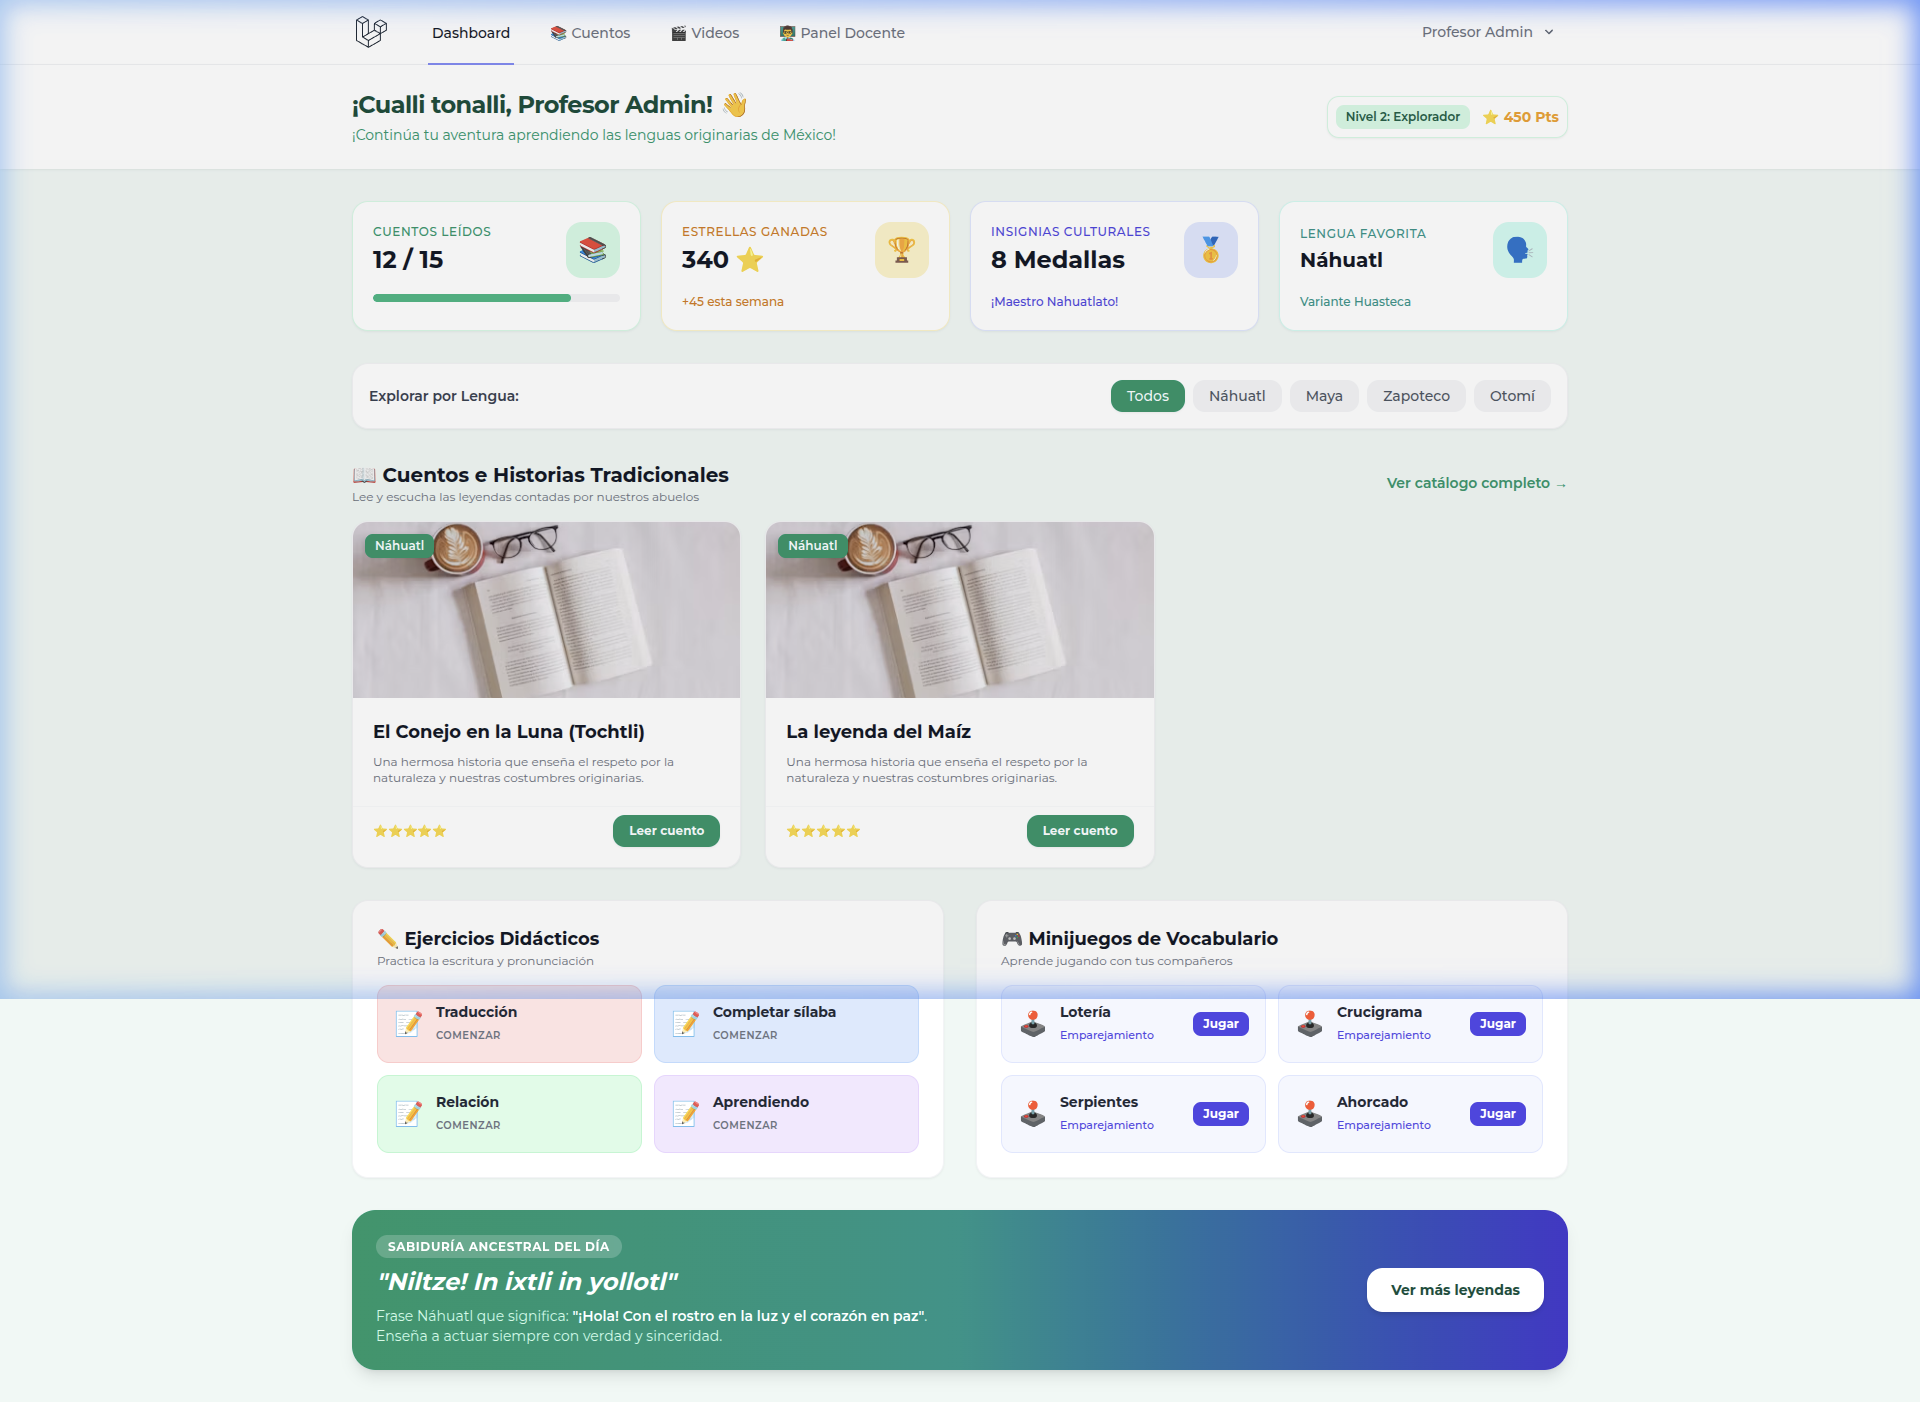
\includegraphics[height=4.2cm]{../img/Interfaces/Student_Main_Menu.png}
            \\[0.3em]
            {\tiny\color{lighttext!60}Menú Principal del Alumno}
        \end{column}
    \end{columns}
\end{frame}

% --- GALERÍA DE INTERFACES: 1 POR DIAPOSITIVA (GRANDE Y SIN DESBORDAMIENTOS) ---

% Slide 5: Interfaz 1
\begin{frame}{Interfaz: Selección de Idioma}
    \begin{tikzpicture}[remember picture,overlay]
        \node[anchor=north east, xshift=-0.3cm, yshift=-0.3cm] at (current page.north east) 
        {
\includegraphics[height=0.3cm]{../img/logos/CS_adjus.png}};
    \end{tikzpicture}
    \centering
    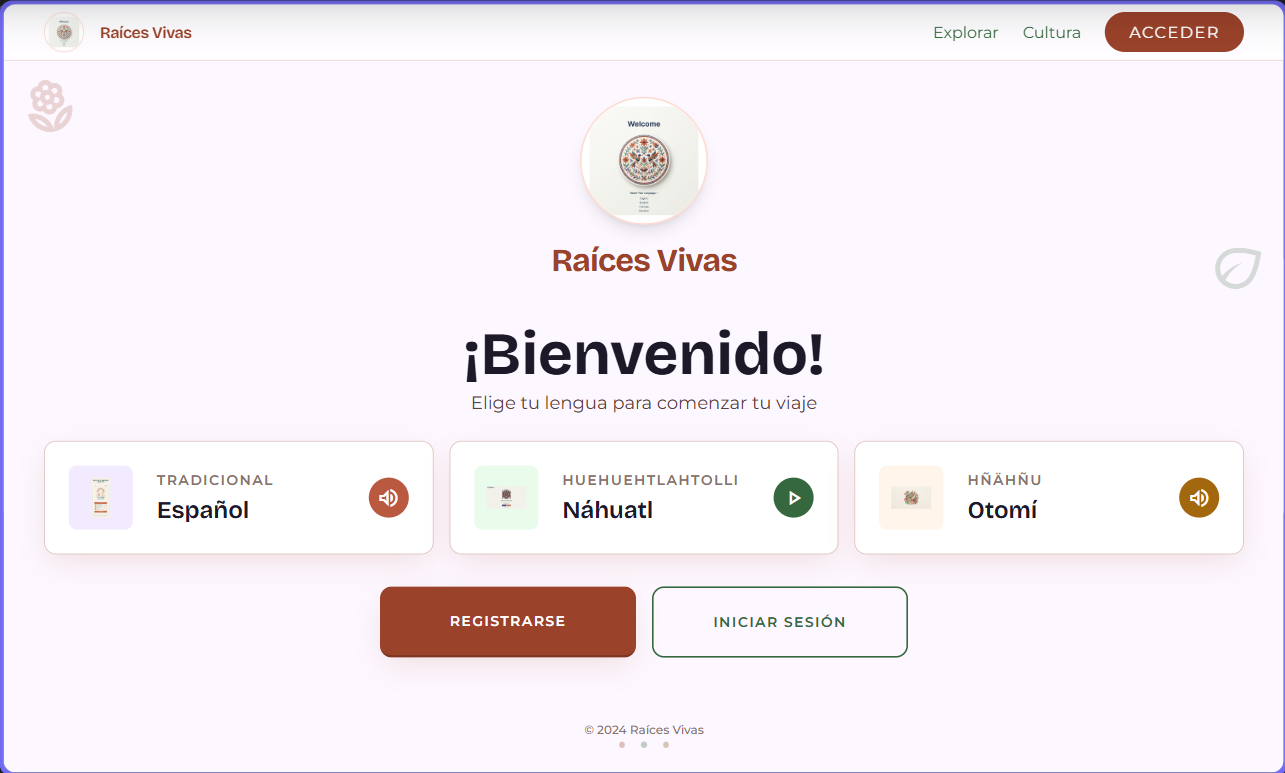
\includegraphics[height=4.8cm]{../img/Interfaces/Welcome__and__Language_Selection.png}
    \par\vspace{0.4em}
    {\small\color{lighttext!70}Pantalla inicial interactiva para niños: Selección de lengua originaria a aprender.}
\end{frame}

% Slide 6: Interfaz 2
\begin{frame}{Interfaz: Inicio de Sesión}
    \begin{tikzpicture}[remember picture,overlay]
        \node[anchor=north east, xshift=-0.3cm, yshift=-0.3cm] at (current page.north east) 
        {
\includegraphics[height=0.3cm]{../img/logos/CS_adjus.png}};
    \end{tikzpicture}
    \centering
    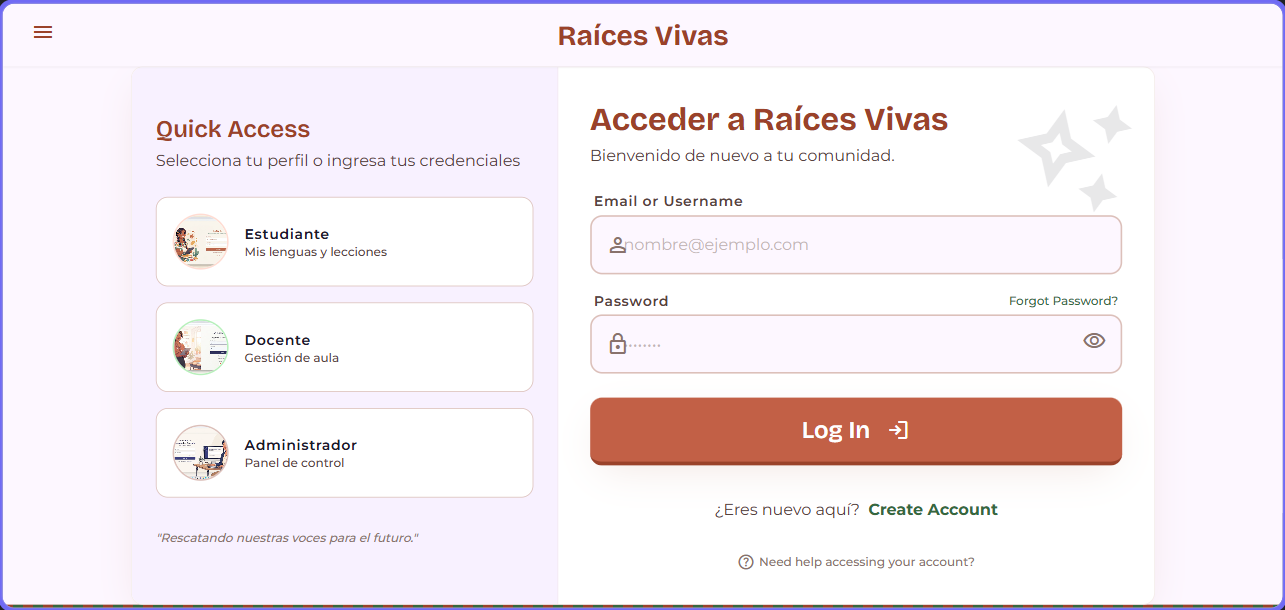
\includegraphics[height=4.8cm]{../img/Interfaces/Log_In.png}
    \par\vspace{0.4em}
    {\small\color{lighttext!70}Pantalla de autenticación para estudiantes, docentes y administradores.}
\end{frame}

% Slide 7: Interfaz 3
\begin{frame}{Interfaz: Registro de Usuario}
    \begin{tikzpicture}[remember picture,overlay]
        \node[anchor=north east, xshift=-0.3cm, yshift=-0.3cm] at (current page.north east) 
        {
\includegraphics[height=0.3cm]{../img/logos/CS_adjus.png}};
    \end{tikzpicture}
    \centering
    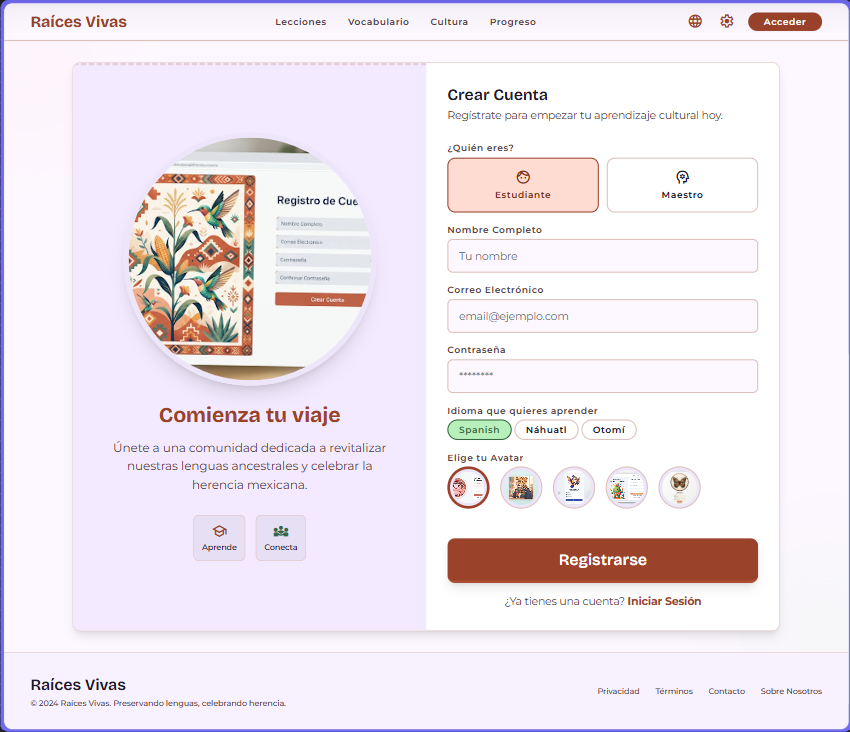
\includegraphics[height=4.8cm]{../img/Interfaces/Registration.png}
    \par\vspace{0.4em}
    {\small\color{lighttext!70}Formulario de registro infantil adaptado visualmente con avatares y campos mínimos.}
\end{frame}

% Slide 8: Interfaz 4
\begin{frame}{Interfaz: Recuperación de Contraseña}
    \begin{tikzpicture}[remember picture,overlay]
        \node[anchor=north east, xshift=-0.3cm, yshift=-0.3cm] at (current page.north east) 
        {
\includegraphics[height=0.3cm]{../img/logos/CS_adjus.png}};
    \end{tikzpicture}
    \centering
    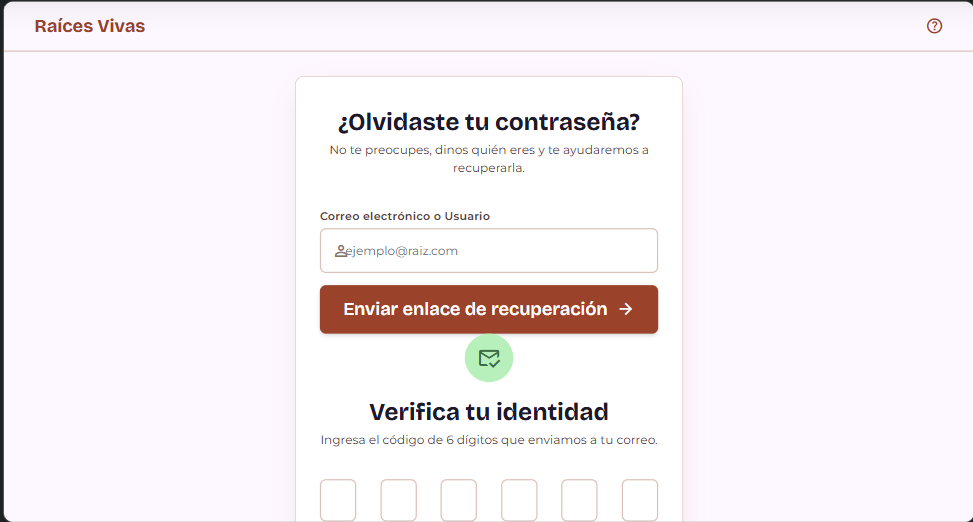
\includegraphics[height=4.8cm]{../img/Interfaces/Password_Recovery.png}
    \par\vspace{0.4em}
    {\small\color{lighttext!70}Formulario para envío seguro de códigos de verificación y restablecimiento de claves.}
\end{frame}

% Slide 9: Interfaz 5
\begin{frame}{Interfaz: Perfil de Usuario}
    \begin{tikzpicture}[remember picture,overlay]
        \node[anchor=north east, xshift=-0.3cm, yshift=-0.3cm] at (current page.north east) 
        {
\includegraphics[height=0.3cm]{../img/logos/CS_adjus.png}};
    \end{tikzpicture}
    \centering
    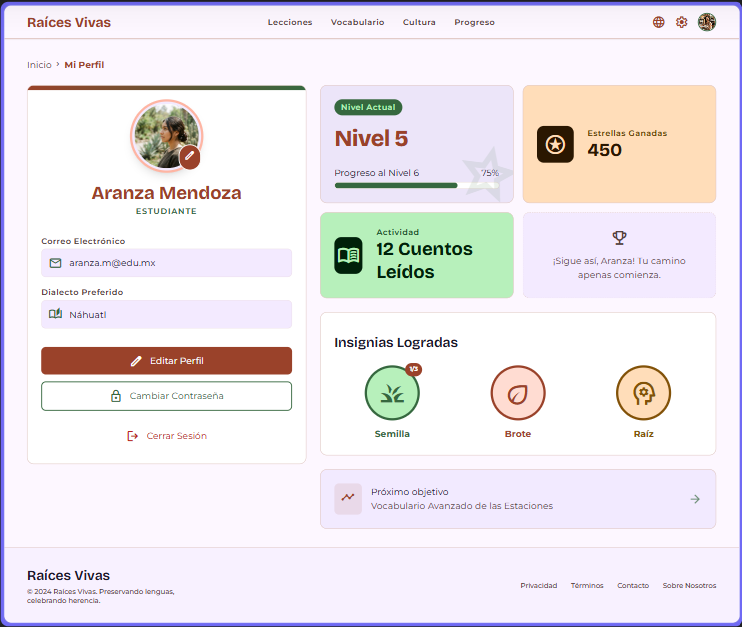
\includegraphics[height=4.8cm]{../img/Interfaces/User_Profile.png}
    \par\vspace{0.4em}
    {\small\color{lighttext!70}Panel del alumno para visualizar avatares seleccionados, información básica e idioma activo.}
\end{frame}

% Slide 10: Interfaz 6
\begin{frame}{Interfaz: Mis Logros y Medallas}
    \begin{tikzpicture}[remember picture,overlay]
        \node[anchor=north east, xshift=-0.3cm, yshift=-0.3cm] at (current page.north east) 
        {
\includegraphics[height=0.3cm]{../img/logos/CS_adjus.png}};
    \end{tikzpicture}
    \centering
    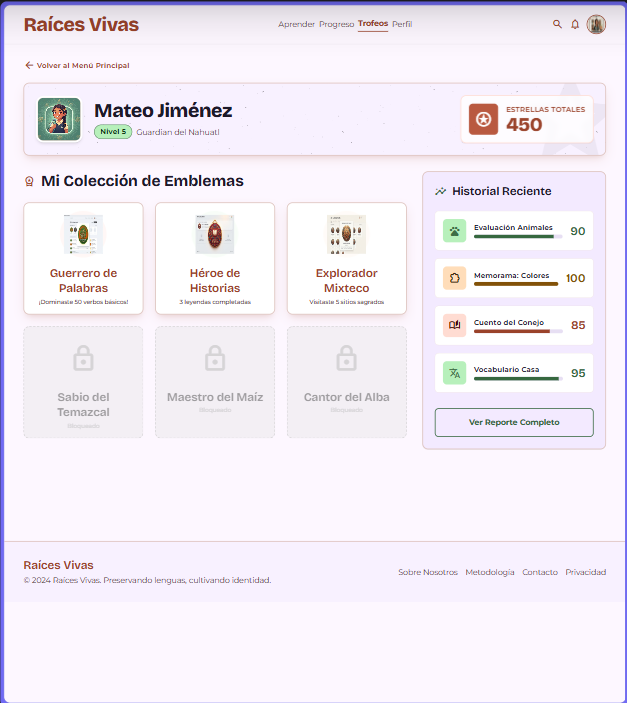
\includegraphics[height=4.8cm]{../img/Interfaces/My_Achievements.png}
    \par\vspace{0.4em}
    {\small\color{lighttext!70}Sistema de gamificación: Medallas obtenidas por cuentos leídos y juegos completados.}
\end{frame}

% Slide 11: Interfaz 7
\begin{frame}{Interfaz: Catálogo de Cuentos}
    \begin{tikzpicture}[remember picture,overlay]
        \node[anchor=north east, xshift=-0.3cm, yshift=-0.3cm] at (current page.north east) 
        {
\includegraphics[height=0.3cm]{../img/logos/CS_adjus.png}};
    \end{tikzpicture}
    \centering
    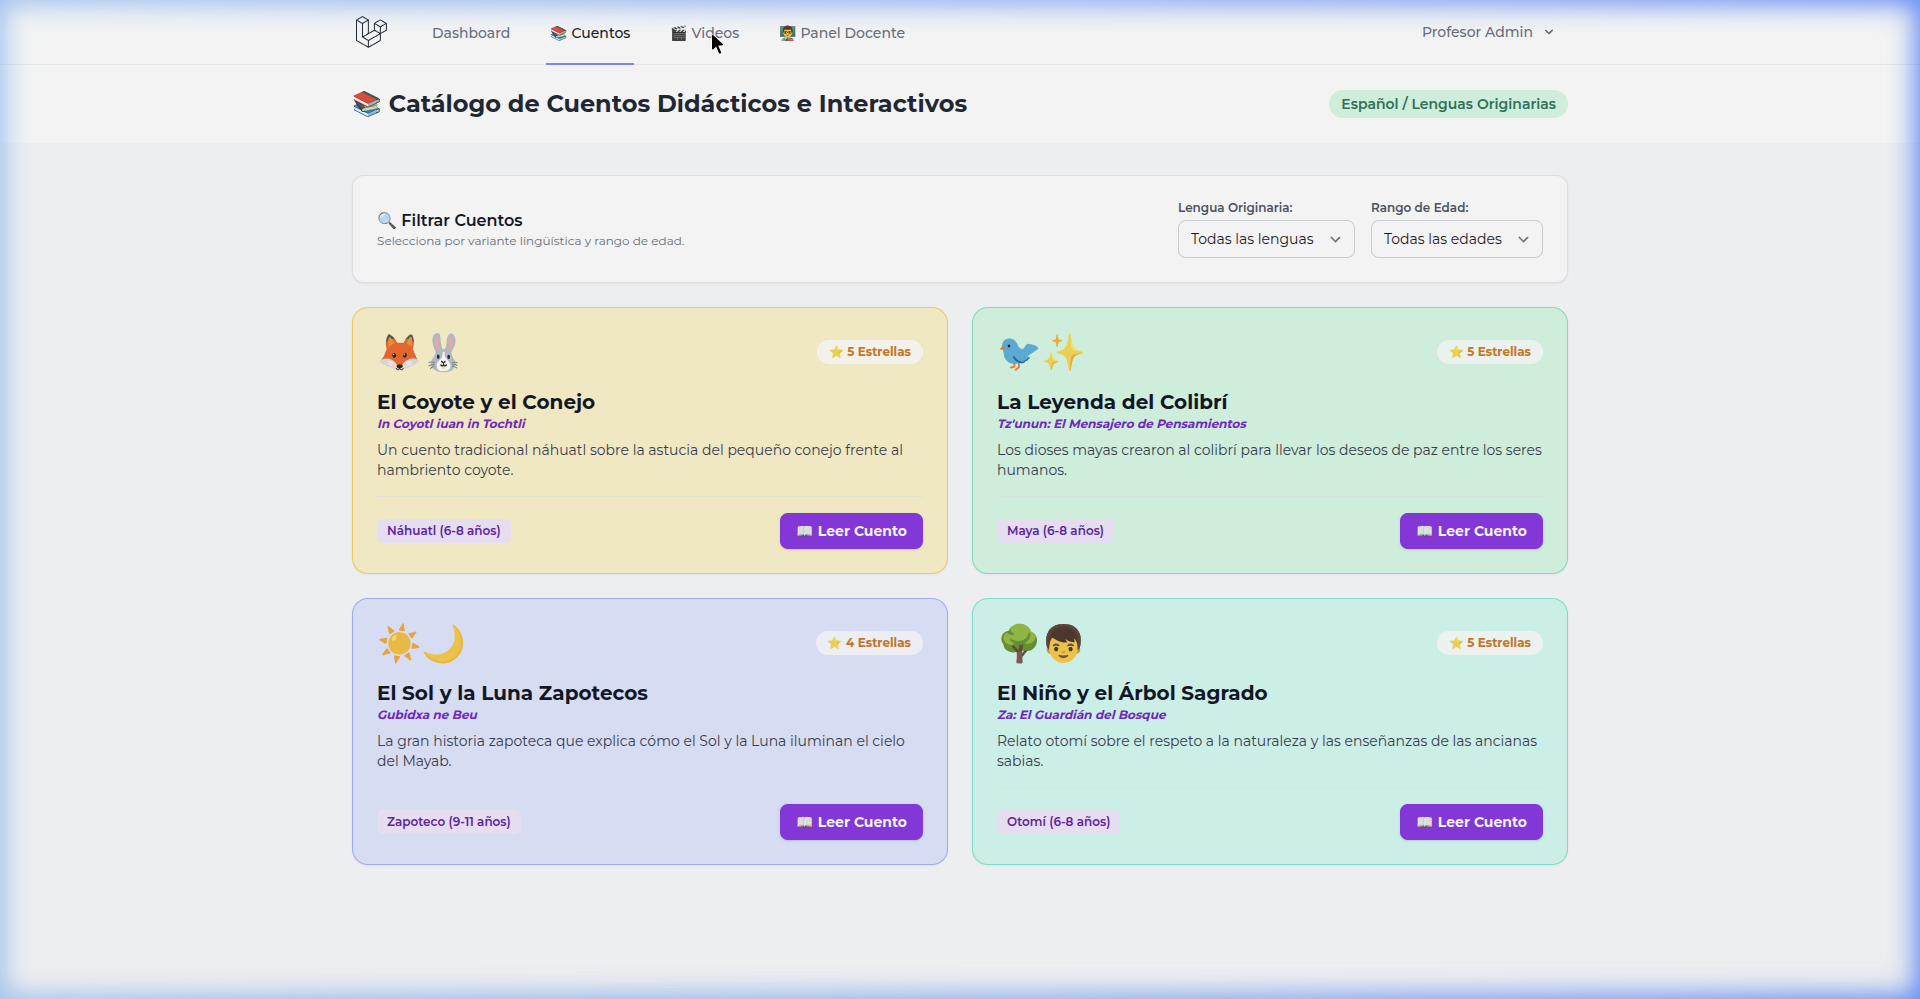
\includegraphics[height=4.8cm]{../img/Interfaces/Stories_Catalog.png}
    \par\vspace{0.4em}
    {\small\color{lighttext!70}Galería de cuentos tradicionales clasificados por categorías temáticas e idiomas.}
\end{frame}

% Slide 12: Interfaz 8
\begin{frame}{Interfaz: Lector de Cuentos Interactivo}
    \begin{tikzpicture}[remember picture,overlay]
        \node[anchor=north east, xshift=-0.3cm, yshift=-0.3cm] at (current page.north east) 
        {
\includegraphics[height=0.3cm]{../img/logos/CS_adjus.png}};
    \end{tikzpicture}
    \centering
    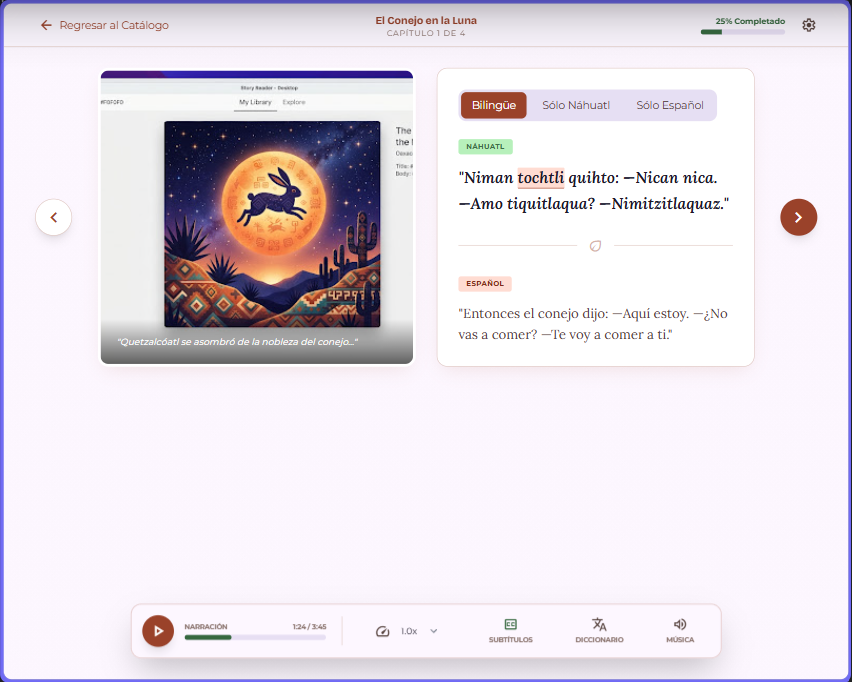
\includegraphics[height=4.8cm]{../img/Interfaces/Story_Reader.png}
    \par\vspace{0.4em}
    {\small\color{lighttext!70}Interfaz de lectura con ilustraciones grandes, narración en audio y traducción en tiempo real.}
\end{frame}

% Slide 13: Interfaz 9
\begin{frame}{Interfaz: Catálogo de Juegos Educativos}
    \begin{tikzpicture}[remember picture,overlay]
        \node[anchor=north east, xshift=-0.3cm, yshift=-0.3cm] at (current page.north east) 
        {
\includegraphics[height=0.3cm]{../img/logos/CS_adjus.png}};
    \end{tikzpicture}
    \centering
    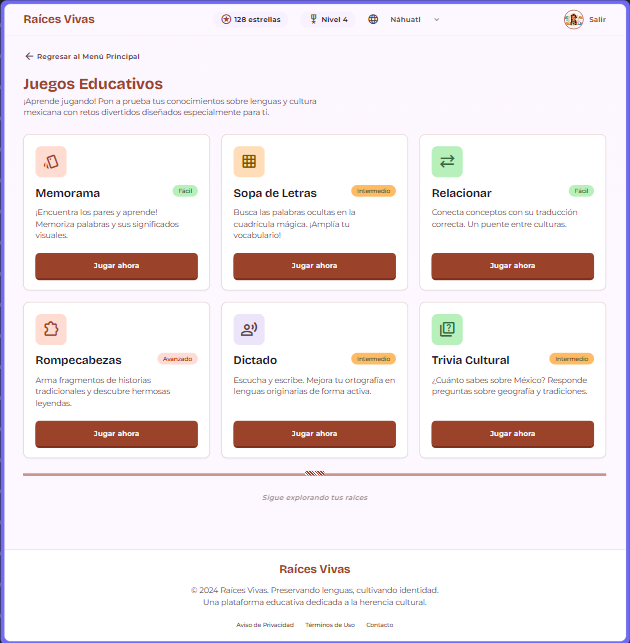
\includegraphics[height=4.8cm]{../img/Interfaces/Educational_Games_Catalog.png}
    \par\vspace{0.4em}
    {\small\color{lighttext!70}Galería con accesos directos a actividades lúdicas de vocabulario y gramática.}
\end{frame}

% Slide 14: Interfaz 10
\begin{frame}{Interfaz: Juego de Memoria (Memorama)}
    \begin{tikzpicture}[remember picture,overlay]
        \node[anchor=north east, xshift=-0.3cm, yshift=-0.3cm] at (current page.north east) 
        {
\includegraphics[height=0.3cm]{../img/logos/CS_adjus.png}};
    \end{tikzpicture}
    \centering
    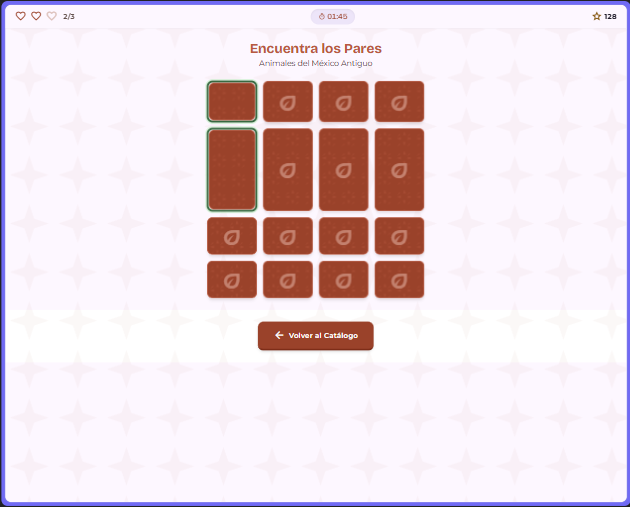
\includegraphics[height=4.8cm]{../img/Interfaces/Memory_Game.png}
    \par\vspace{0.4em}
    {\small\color{lighttext!70}Actividad interactiva de emparejar palabras en español y lengua originaria mediante tarjetas.}
\end{frame}

% Slide 15: Interfaz 11
\begin{frame}{Interfaz: Juego de Relacionar Palabras}
    \begin{tikzpicture}[remember picture,overlay]
        \node[anchor=north east, xshift=-0.3cm, yshift=-0.3cm] at (current page.north east) 
        {
\includegraphics[height=0.3cm]{../img/logos/CS_adjus.png}};
    \end{tikzpicture}
    \centering
    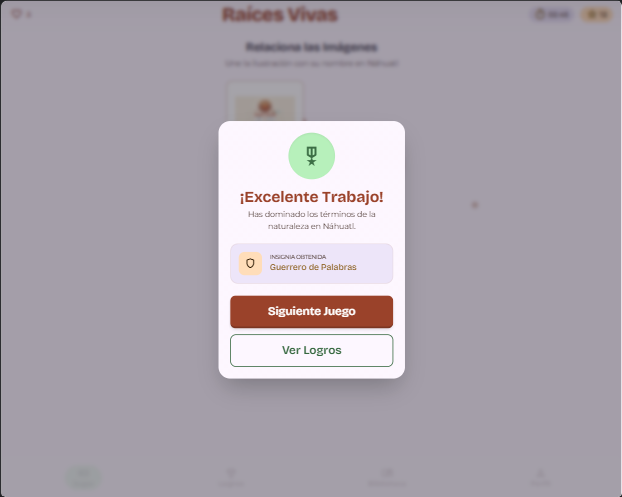
\includegraphics[height=4.8cm]{../img/Interfaces/Word_Matching_Game.png}
    \par\vspace{0.4em}
    {\small\color{lighttext!70}Juego interactivo para trazar líneas de correspondencia semántica entre palabras e imágenes.}
\end{frame}

% Slide 16: Interfaz 12
\begin{frame}{Interfaz: Menú Principal del Alumno}
    \begin{tikzpicture}[remember picture,overlay]
        \node[anchor=north east, xshift=-0.3cm, yshift=-0.3cm] at (current page.north east) 
        {
\includegraphics[height=0.3cm]{../img/logos/CS_adjus.png}};
    \end{tikzpicture}
    \centering
    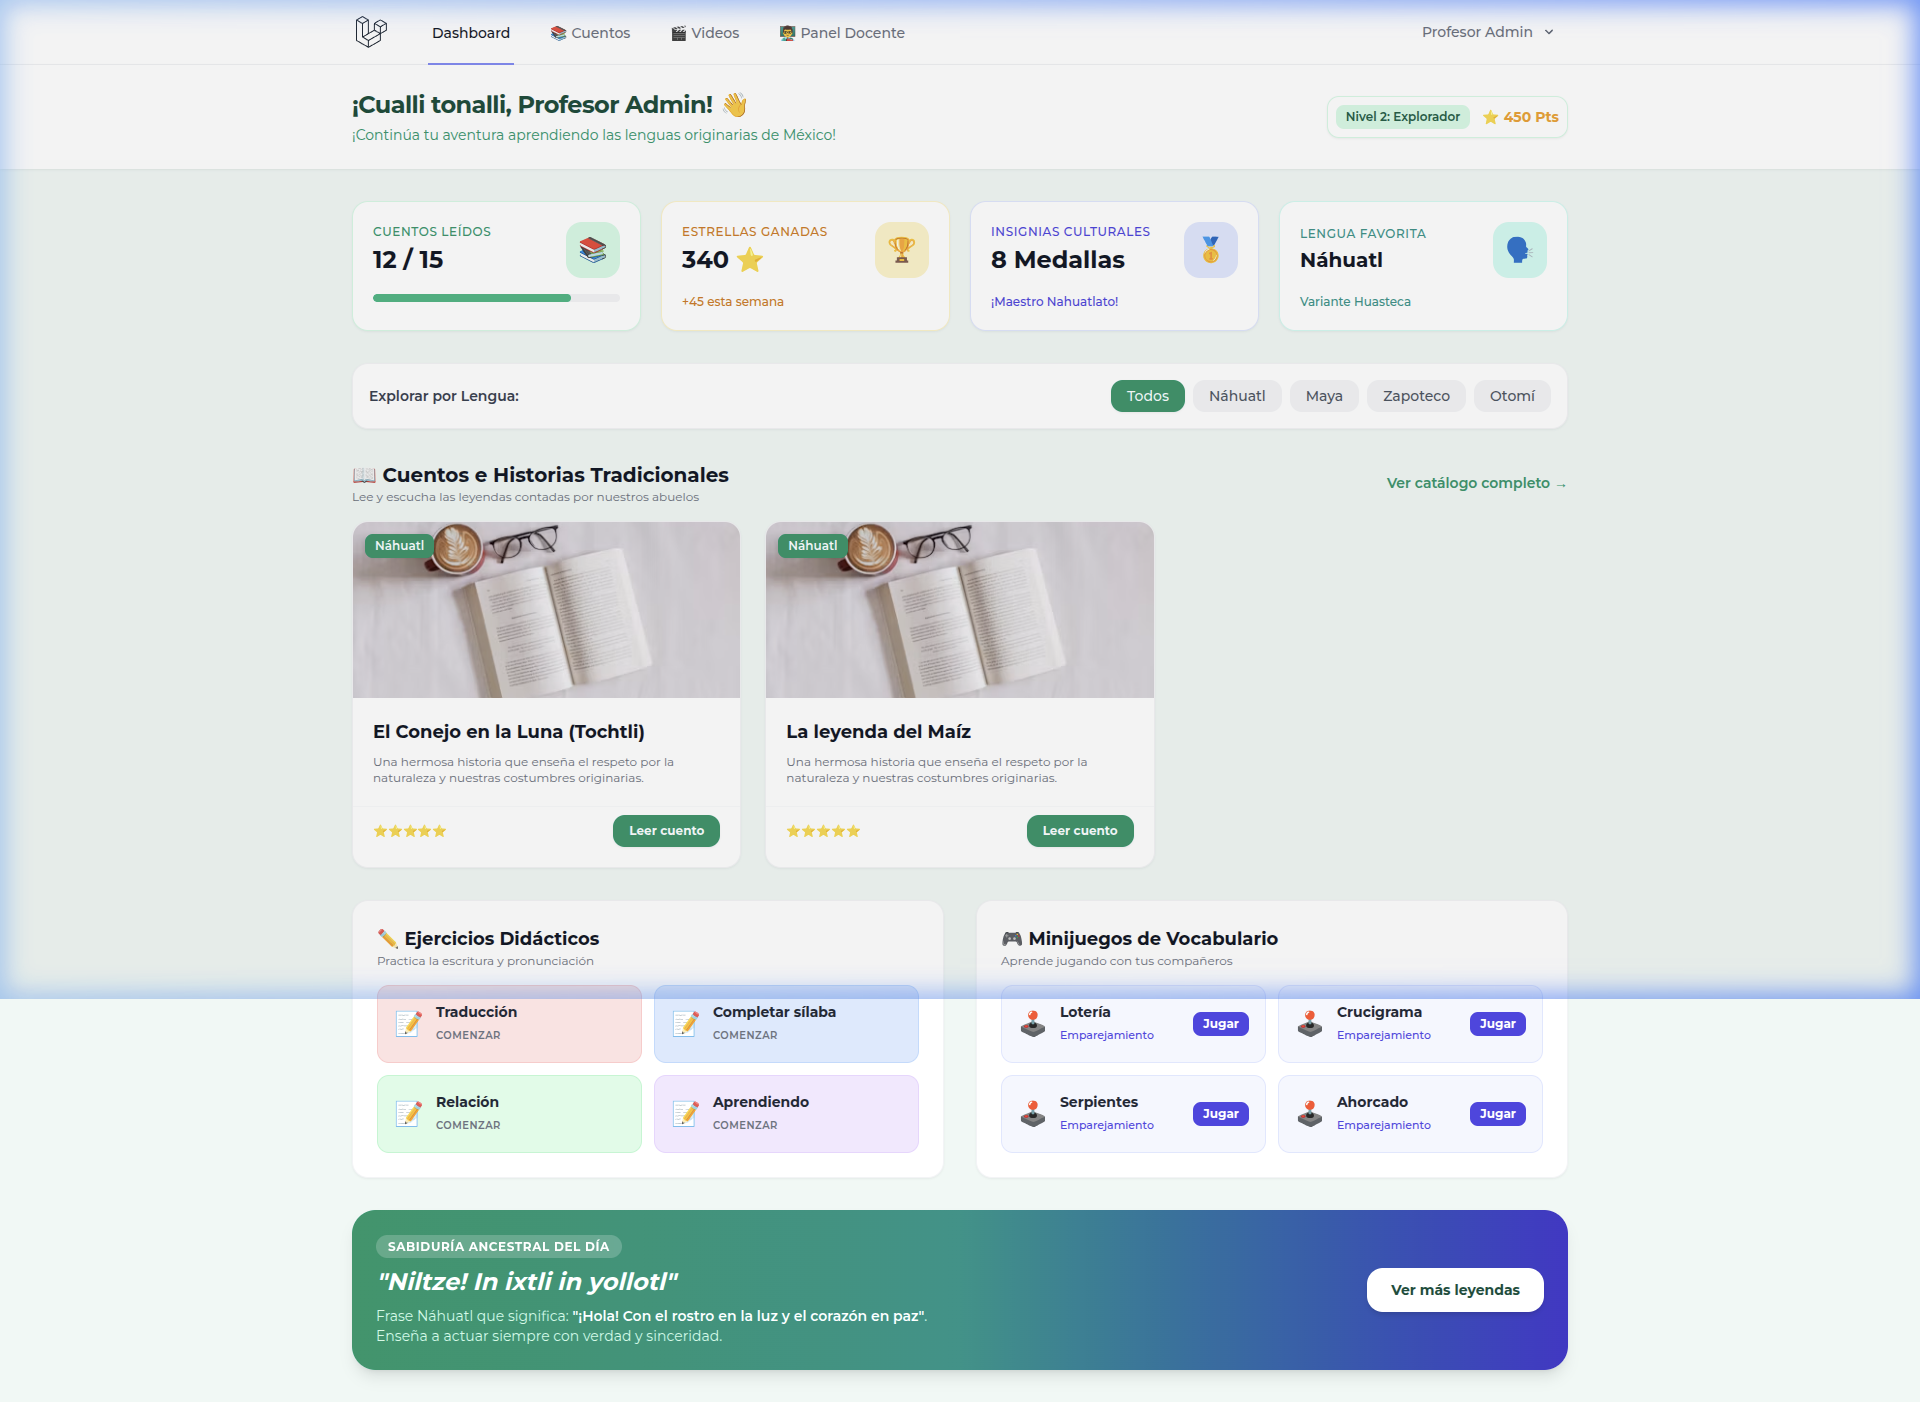
\includegraphics[height=4.8cm]{../img/Interfaces/Student_Main_Menu.png}
    \par\vspace{0.4em}
    {\small\color{lighttext!70}Panel principal con acceso unificado a cuentos, juegos, perfil y progreso acumulativo.}
\end{frame}

% Slide 17: Parte 2 - Título
\begin{frame}[plain]
    \begin{tikzpicture}[remember picture,overlay]
        \node[anchor=north east, xshift=-0.3cm, yshift=-0.3cm] at (current page.north east) 
        {
\includegraphics[height=0.3cm]{../img/logos/CS_adjus.png}};
        \node[text=techblue, opacity=0.03, font=\bfseries, scale=35] at (current page.center) {2};
    \end{tikzpicture}
    \centering
    \vspace{2.2cm}
    {\huge\bfseries\color{techblue}PARTE 2: DIAGNÓSTICO}\\[0.2em]
    {\huge\bfseries\color{techblue}Y ANÁLISIS ESTÁTICO}
\end{frame}

% Slide 18: Parte 2 - SonarQube
\begin{frame}{Diagnóstico Estático con SonarQube}
    \begin{tikzpicture}[remember picture,overlay]
        \node[anchor=north east, xshift=-0.3cm, yshift=-0.3cm] at (current page.north east) 
        {
\includegraphics[height=0.3cm]{../img/logos/CS_adjus.png}};
    \end{tikzpicture}
    \begin{columns}[onlytextwidth,c]
        \begin{column}{0.45\textwidth}
            \textbf{Análisis de Calidad}
            \begin{itemize}
                \item Auditoría con \textbf{SonarQube v25.2.0} en PHP y JavaScript.
            \end{itemize}
            \vspace{0.3em}
            \textbf{Métricas y Hallazgos}
            \begin{itemize}
                \item \textbf{Fiabilidad C}: 67 bugs (1 Alta severidad, 6 Media).
                \item \textbf{115 Code Smells}: Deuda de \textbf{6h 54m}.
            \end{itemize}
        \end{column}
        
        \begin{column}{0.5\textwidth}
            \centering
            % Visual Dashboard Schema
            \begin{tikzpicture}[
                scale=1.0, transform shape,
                card/.style={draw=techblue!30, fill=cardbg, thick, rounded corners=6pt},
                badge/.style={circle, minimum size=0.6cm, font=\bfseries\small, text=white, align=center, inner sep=0pt}
            ]
                % Contenedor principal
                \draw[card] (0, -2.2) rectangle (6.2, 1.2);
                
                % Título del Card
                \node[font=\footnotesize\bfseries\color{techblue}, anchor=west] at (0.3, 0.8) {AUDITORÍA SONARQUBE};
                
                % Columna 1: Bugs
                \node[font=\tiny\color{lighttext!60}, anchor=west] at (0.4, 0.2) {BUGS};
                \node[font=\LARGE\bfseries\color{accentred}, anchor=west] at (0.4, -0.4) {67};
                \node[badge, fill=accentorange, label={right:\tiny\color{lighttext}Rating C}] (r1) at (0.8, -1.3) {C};
                
                % Columna 2: Seguridad
                \node[font=\tiny\color{lighttext!60}, anchor=west] at (2.4, 0.2) {SEGURIDAD};
                \node[font=\LARGE\bfseries\color{accentgreen}, anchor=west] at (2.4, -0.4) {0};
                \node[badge, fill=accentgreen, label={right:\tiny\color{lighttext}Rating A}] (r2) at (2.8, -1.3) {A};
                
                % Columna 3: Code Smells
                \node[font=\tiny\color{lighttext!60}, anchor=west] at (4.4, 0.2) {DEUDA};
                \node[font=\LARGE\bfseries\color{accentgreen}, anchor=west] at (4.4, -0.4) {115};
                \node[badge, fill=accentgreen, label={right:\tiny\color{lighttext}Rating A}] (r3) at (4.8, -1.3) {A};
                
                % Líneas divisoras
                \draw[techblue!20, thin] (2.1, 0.3) -- (2.1, -1.8);
                \draw[techblue!20, thin] (4.1, 0.3) -- (4.1, -1.8);
            \end{tikzpicture}
        \end{column}
    \end{columns}
\end{frame}

% Slide 19: Parte 2 - Incidente Crítico
\begin{frame}{Incidente Crítico: Reconstitución (PR-001)}
    \begin{tikzpicture}[remember picture,overlay]
        \node[anchor=north east, xshift=-0.3cm, yshift=-0.3cm] at (current page.north east) 
        {
\includegraphics[height=0.3cm]{../img/logos/CS_adjus.png}};
    \end{tikzpicture}
    \begin{columns}[onlytextwidth,c]
        \begin{column}{0.48\textwidth}
            \small
            \textbf{Fallo del Entregable Original}
            \begin{itemize}
                \item Ausencia total de \path{resources/js/Pages/}, lo que impedía levantar las vistas React.
                \item Error 500 generalizado en el servidor por falta de assets compilados.
            \end{itemize}
            \vspace{0.2em}
            \textbf{Resolución Aplicada}
            \begin{itemize}
                \item Reconstitución del entorno de desarrollo, configuración de Vite y reconstrucción de componentes.
            \end{itemize}
        \end{column}
        
        \begin{column}{0.48\textwidth}
            \centering
            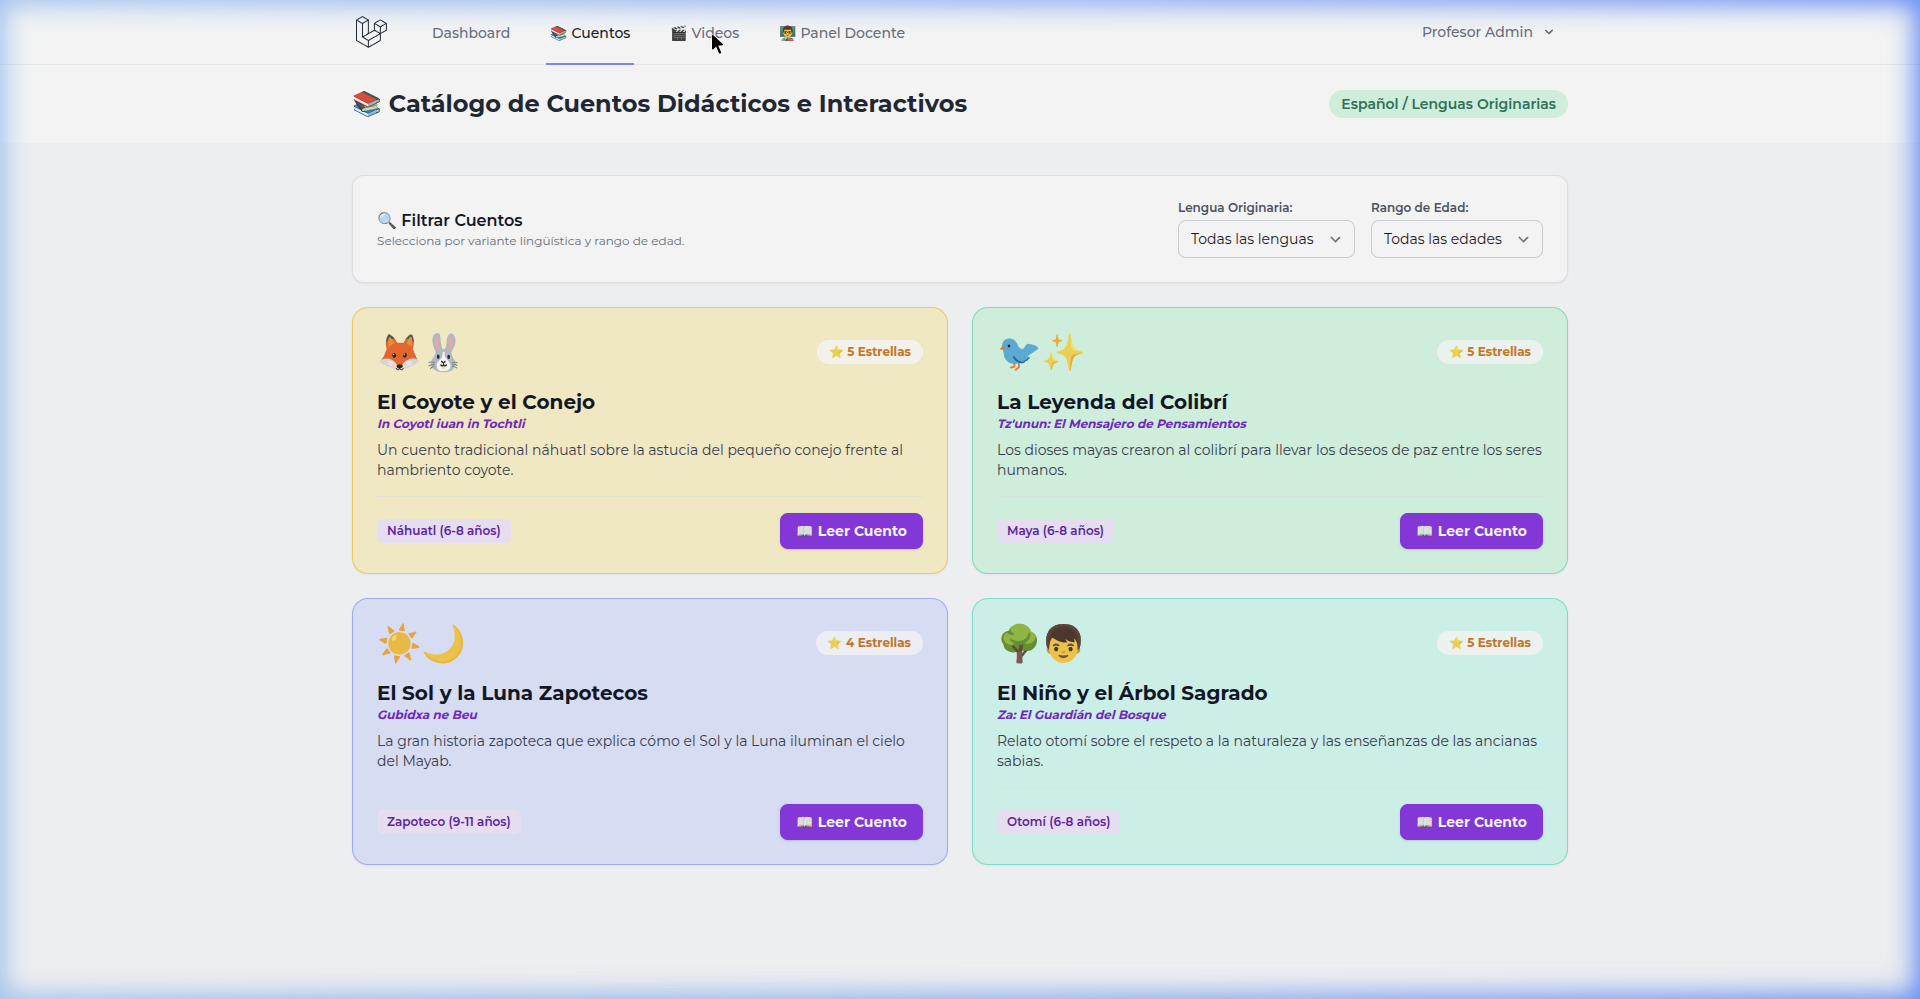
\includegraphics[height=4.2cm]{../img/Interfaces/Stories_Catalog.png}
            \\[0.3em]
            {\tiny\color{lighttext!60}Catálogo de Cuentos Reconstituido}
        \end{column}
    \end{columns}
\end{frame}

% Slide 20: Parte 3 - Título
\begin{frame}[plain]
    \begin{tikzpicture}[remember picture,overlay]
        \node[anchor=north east, xshift=-0.3cm, yshift=-0.3cm] at (current page.north east) 
        {
\includegraphics[height=0.3cm]{../img/logos/CS_adjus.png}};
        \node[text=techblue, opacity=0.03, font=\bfseries, scale=35] at (current page.center) {3};
    \end{tikzpicture}
    \centering
    \vspace{2.2cm}
    {\huge\bfseries\color{techblue}PARTE 3: PRUEBAS,}\\[0.2em]
    {\huge\bfseries\color{techblue}PR/MR Y MÉTRICAS DEL PROCESO}
\end{frame}

% Slide 21: Resultados de Pruebas Funcionales - Diagnóstico Inicial
\begin{frame}{Pruebas Funcionales: Diagnóstico Inicial}
    \begin{tikzpicture}[remember picture,overlay]
        \node[anchor=north east, xshift=-0.3cm, yshift=-0.3cm] at (current page.north east) 
        {
\includegraphics[height=0.3cm]{../img/logos/CS_adjus.png}};
    \end{tikzpicture}
    \begin{columns}[onlytextwidth,c]
        \begin{column}{0.5\textwidth}
            \textbf{Auditoría de Caja Negra (v1.0.0)}
            \begin{itemize}
                \item Pruebas funcionales de extremo a extremo.
                \item \textbf{Éxito inicial}: 6/8 casos aprobados (75\%).
            \end{itemize}
            \vspace{0.5em}
            \textbf{Fallas Críticas Identificadas}
            \begin{itemize}
                \item \textbf{CP007 (Fallo)}: Filtro de búsqueda de cuentos inoperante.
                \item \textbf{CP008 (Fallo)}: Avance y progreso infantil no persistidos en base de datos.
            \end{itemize}
        \end{column}
        
        \begin{column}{0.48\textwidth}
            \centering
            \begin{tikzpicture}[scale=1.0]
                \fill[cardbg] (-1.8,-1.8) rectangle (1.8,1.8);
                % Donut chart
                \draw[accentred, line width=7pt] (0,0) circle (1.0cm);
                \draw[accentgreen, line width=7.2pt] (0,0) ++(90:1.0cm) arc (90:-180:1.0cm); % 75%
                
                % Center labels
                \node[font=\tiny\bfseries\color{white}] at (0,0.15) {8 CASOS};
                \node[font=\tiny\color{lighttext!60}] at (0,-0.15) {DE PRUEBA};
                
                % Legend
                \node[anchor=west, font=\tiny\color{accentgreen}] at (1.8,0.4) {\statusdot{accentgreen} 6 Aprobados (75\%)};
                \node[anchor=west, font=\tiny\color{accentred}] at (1.8,-0.4) {\statusdot{accentred} 2 Fallidos (25\%)};
            \end{tikzpicture}
        \end{column}
    \end{columns}
\end{frame}

% Slide 22: Resultados de Pruebas Funcionales - Remediación y Cierre
\begin{frame}{Pruebas Funcionales: Remediación y Cierre}
    \begin{tikzpicture}[remember picture,overlay]
        \node[anchor=north east, xshift=-0.3cm, yshift=-0.3cm] at (current page.north east) 
        {
\includegraphics[height=0.3cm]{../img/logos/CS_adjus.png}};
    \end{tikzpicture}
    \begin{columns}[onlytextwidth,c]
        \begin{column}{0.52\textwidth}
            \textbf{Acciones de Corrección}
            \begin{itemize}
                \item \textbf{Remediación del Filtro (MR-004)}: Reconstrucción de la lógica de Laravel Eloquent en controladores.
                \item \textbf{Remediación del Progreso (MR-005)}: Implementación de endpoints y base de datos PostgreSQL para almacenar el progreso de los alumnos.
            \end{itemize}
            \vspace{0.4em}
            \textbf{Resultados de Regresión}
            \begin{itemize}
                \item Re-ejecución total de los 8 casos de prueba.
                \item \textbf{Cobertura de pruebas exitosas}: 100\% (8/8 aprobados).
            \end{itemize}
        \end{column}
        
        \begin{column}{0.45\textwidth}
            \centering
            \begin{tikzpicture}[scale=1.0]
                \fill[cardbg] (-1.8,-1.8) rectangle (1.8,1.8);
                % Donut chart (100% Green)
                \draw[accentgreen, line width=7.2pt] (0,0) circle (1.0cm);
                
                % Center labels
                \node[font=\tiny\bfseries\color{white}] at (0,0.15) {100\%};
                \node[font=\tiny\color{lighttext!60}] at (0,-0.15) {APROBADO};
                
                % Legend
                \node[anchor=west, font=\tiny\color{accentgreen}] at (1.8,0) {\statusdot{accentgreen} 8 Aprobados (100\%)};
            \end{tikzpicture}
        \end{column}
    \end{columns}
\end{frame}

% Slide 22: Reporte de Problemas
\begin{frame}{Problem Reports (PR) y Solicitudes de Modificación}
    \begin{tikzpicture}[remember picture,overlay]
        \node[anchor=north east, xshift=-0.3cm, yshift=-0.3cm] at (current page.north east) 
        {
\includegraphics[height=0.3cm]{../img/logos/CS_adjus.png}};
    \end{tikzpicture}
    \centering\scriptsize
    \renewcommand{\arraystretch}{1.1}
    \begin{table}
        \color{lighttext}
        \begin{tabularx}{\textwidth}{llcX}
            \toprule
            \textbf{ID MR} & \textbf{Incidente Asociado} & \textbf{Prioridad} & \textbf{Solución Técnica en el Plan} \\
            \midrule
            \textbf{MR-001} & PR-001 (Ausencia Frontend)   & \statusdot{accentred} Crítica & Reconstituir las vistas React e integrarlas en Laravel. \\
            \textbf{MR-002} & PR-002 (67 Bugs de tipado)   & \statusdot{accentorange} Alta & Corregir lógica de datos y tipado en frontend. \\
            \textbf{MR-003} & PR-003 (115 Code Smells)    & \statusdot{techblue} Baja & Integrar linters automáticos locales (PHP-CS-Fixer y ESLint). \\
            \textbf{MR-004} & PR-004 (Fallas en Filtro CP007) & \statusdot{accentorange} Media & Agregar cláusulas condicionales de filtrado en controladores. \\
            \textbf{MR-005} & PR-005 (Falla Progreso CP008) & \statusdot{accentred} Alta & Crear persistencia en base de datos para progreso infantil. \\
            \bottomrule
        \end{tabularx}
    \end{table}
\end{frame}

% --- EXPANSIÓN DE MÉTRICAS (AE8) ---

% Slide 23: Métricas - MTTR y EPR
\begin{frame}{Métricas: Resolución Temporal y Efectividad}
    \begin{tikzpicture}[remember picture,overlay]
        \node[anchor=north east, xshift=-0.3cm, yshift=-0.3cm] at (current page.north east) 
        {
\includegraphics[height=0.3cm]{../img/logos/CS_adjus.png}};
    \end{tikzpicture}
    \begin{columns}[onlytextwidth,c]
        \begin{column}{0.48\textwidth}
            \textbf{Tiempo Medio de Resolución (MTTR-MR)}
            \begin{itemize}
                \item \textbf{Definición:} Mide la rapidez del equipo ante solicitudes de mantenimiento.
                \item \textbf{Resultado:} \textbf{17.78 horas} promedio por cambio (umbral aceptable $< 24$h).
            \end{itemize}
            \begin{block}{Fórmula MTTR-MR}
                \centering\small
                $\text{MTTR-MR} = \frac{\sum_{i=1}^{N} (T_{r, i} - T_{a, i})}{N}$
            \end{block}
        \end{column}
        
        \begin{column}{0.48\textwidth}
            \textbf{Eficacia de Pruebas de Regresión (EPR)}
            \begin{itemize}
                \item \textbf{Definición:} Evalúa si los cambios introdujeron nuevos fallos que llegaron a producción.
                \item \textbf{Resultado:} \textbf{100\%} de efectividad (fuga cero de bugs en el despliegue).
            \end{itemize}
            \begin{block}{Fórmula EPR}
                \centering\small
                $\text{EPR} = \frac{B_{\text{det}}}{B_{\text{det}} + B_{\text{fuga}}} \times 100$
            \end{block}
        \end{column}
    \end{columns}
\end{frame}

% Slide 24: Métricas - PRDT e IM
\begin{frame}{Métricas: Deuda Técnica y Mantenibilidad}
    \begin{tikzpicture}[remember picture,overlay]
        \node[anchor=north east, xshift=-0.3cm, yshift=-0.3cm] at (current page.north east) 
        {
\includegraphics[height=0.3cm]{../img/logos/CS_adjus.png}};
    \end{tikzpicture}
    \begin{columns}[onlytextwidth,c]
        \begin{column}{0.48\textwidth}
            \textbf{Remediación de Deuda Técnica (PRDT)}
            \begin{itemize}
                \item \textbf{Definición:} Proporción de smells y malas prácticas resueltos respecto al diagnóstico inicial.
                \item \textbf{Resultado:} \textbf{95.65\%} (110 de 115 code smells corregidos).
            \end{itemize}
            \begin{block}{Fórmula PRDT}
                \centering\small
                $\text{PRDT} = \frac{D_{\text{rem}}}{D_{\text{tot}}} \times 100$
            \end{block}
        \end{column}
        
        \begin{column}{0.48\textwidth}
            \textbf{Índice de Mantenibilidad (IM)}
            \begin{itemize}
                \item \textbf{Definición:} Métrica estandarizada que califica la viabilidad evolutiva del código base.
                \item \textbf{Resultado:} \textbf{44.82 pts} (Mantenibilidad moderada, estructura estabilizada).
            \end{itemize}
            \begin{block}{Fórmula del Índice (IM)}
                \centering\scriptsize
                $\text{IM} = 171 - 5.2 \ln(V) - 0.23(G) - 16.2 \ln(\text{LOC})$
            \end{block}
        \end{column}
    \end{columns}
\end{frame}

% Slide 25: Métricas - Desglose del IM y Halstead
\begin{frame}{Mantenibilidad: Rangos e Interpretación Técnica}
    \begin{tikzpicture}[remember picture,overlay]
        \node[anchor=north east, xshift=-0.3cm, yshift=-0.3cm] at (current page.north east) 
        {
\includegraphics[height=0.3cm]{../img/logos/CS_adjus.png}};
    \end{tikzpicture}
    \begin{columns}[onlytextwidth,c]
        \begin{column}{0.5\textwidth}
            \small
            \textbf{Componentes de la Ecuación IM}
            \begin{itemize}
                \item \textbf{Volumen de Halstead ($V$):} Mide la complejidad léxica según operadores y operandos.
                \item \textbf{Complejidad Ciclomática ($G$):} Mide el número de caminos lineales independientes en el flujo del código.
                \item \textbf{Líneas de Código (LOC):} Tamaño físico.
            \end{itemize}
        \end{column}
        
        \begin{column}{0.48\textwidth}
            \small
            \textbf{Interpretación de Umbrales (IM)}
            \begin{itemize}
                \item \statusdot{accentgreen} \textbf{IM $\ge 85$}: Alta Mantenibilidad (código limpio, modular, documentado).
                \item \statusdot{accentorange} \textbf{IM $65-84$}: Mantenibilidad Moderada.
                \item \statusdot{accentred} \textbf{IM $< 65$}: Mantenibilidad Crítica (alta deuda, monolítico). Yoliztli se ubica en un rango estable bajo supervisión de linters.
            \end{itemize}
        \end{column}
    \end{columns}
\end{frame}

% --- GALERÍA DE INTERFACES ADM/TEACHER: 1 POR DIAPOSITIVA (GRANDE) ---

% Slide 26: Interfaz 13
\begin{frame}{Interfaz: Dashboard del Docente}
    \begin{tikzpicture}[remember picture,overlay]
        \node[anchor=north east, xshift=-0.3cm, yshift=-0.3cm] at (current page.north east) 
        {
\includegraphics[height=0.3cm]{../img/logos/CS_adjus.png}};
    \end{tikzpicture}
    \centering
    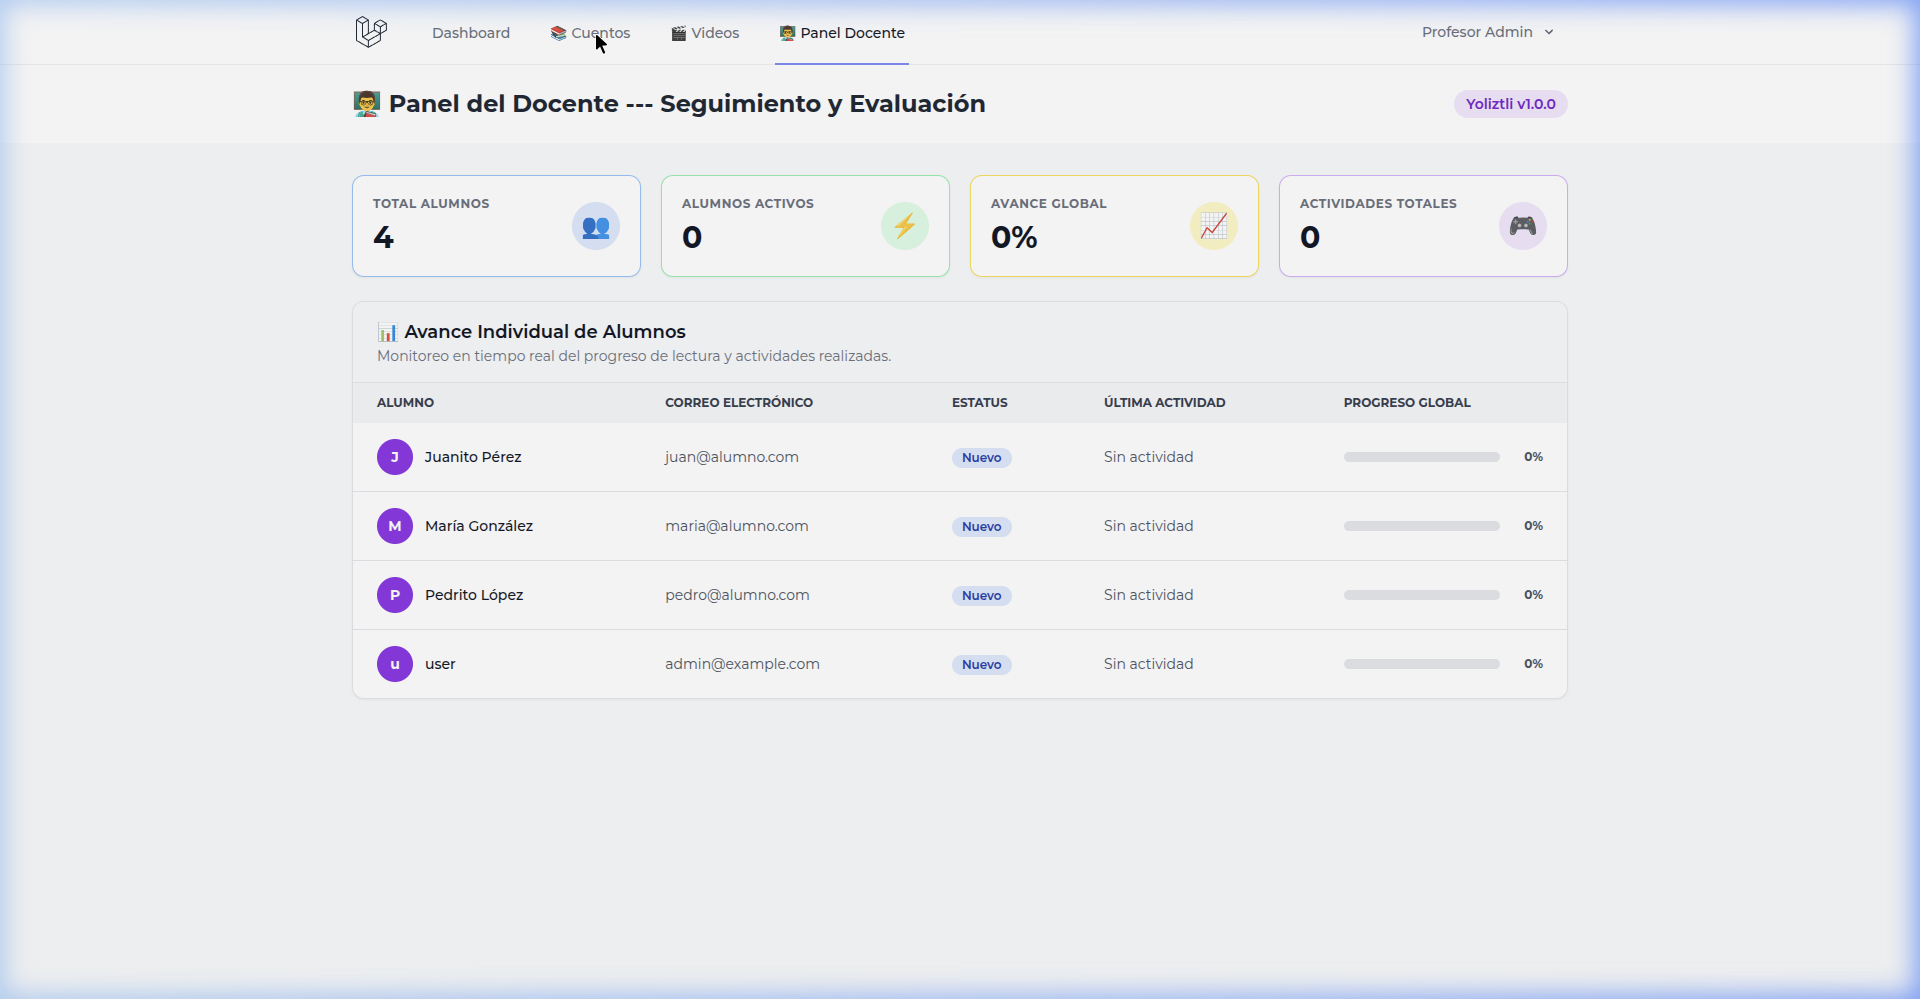
\includegraphics[height=4.8cm]{../img/Interfaces/Teacher_Main_Dashboard.png}
    \par\vspace{0.4em}
    {\small\color{lighttext!70}Consola de control para profesores: Monitoreo de grupos y accesos rápidos a evaluaciones.}
\end{frame}

% Slide 27: Interfaz 14
\begin{frame}{Interfaz: Reportes de Progreso}
    \begin{tikzpicture}[remember picture,overlay]
        \node[anchor=north east, xshift=-0.3cm, yshift=-0.3cm] at (current page.north east) 
        {
\includegraphics[height=0.3cm]{../img/logos/CS_adjus.png}};
    \end{tikzpicture}
    \centering
    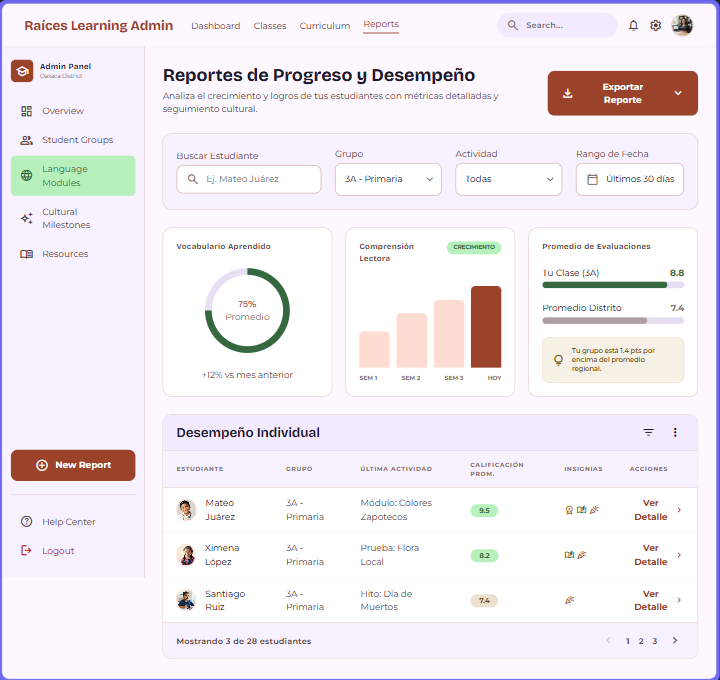
\includegraphics[height=4.8cm]{../img/Interfaces/Reports_Progress_Tracking.png}
    \par\vspace{0.4em}
    {\small\color{lighttext!70}Módulo analítico: Seguimiento del porcentaje de avance en cuentos y juegos por alumno.}
\end{frame}

% Slide 28: Interfaz 15
\begin{frame}{Interfaz: Evaluación del Estudiante}
    \begin{tikzpicture}[remember picture,overlay]
        \node[anchor=north east, xshift=-0.3cm, yshift=-0.3cm] at (current page.north east) 
        {
\includegraphics[height=0.3cm]{../img/logos/CS_adjus.png}};
    \end{tikzpicture}
    \centering
    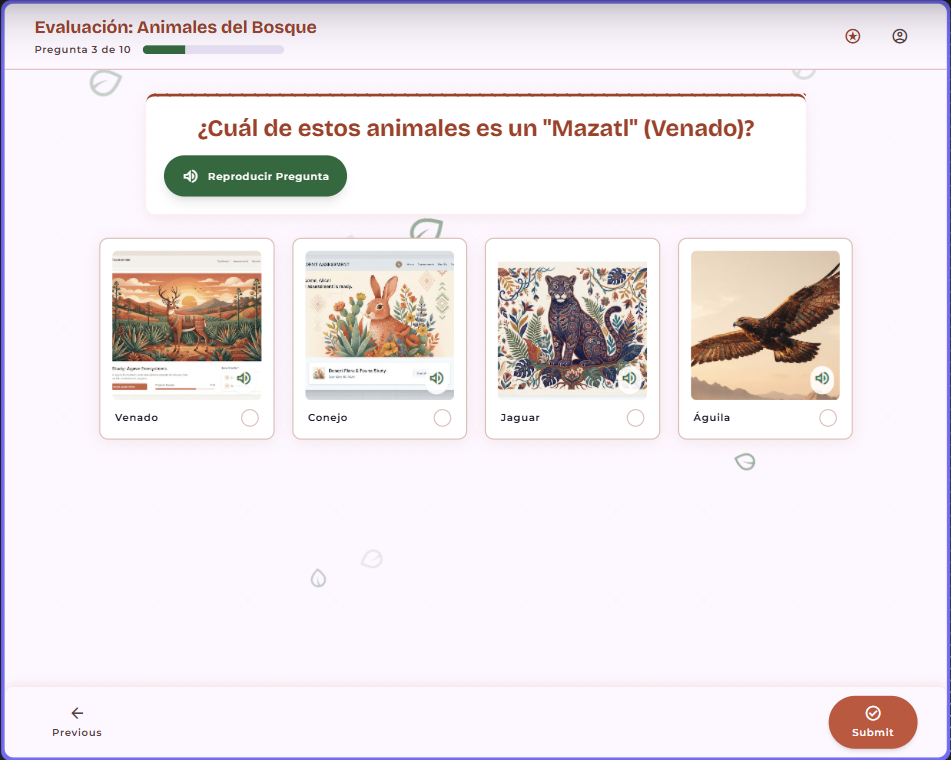
\includegraphics[height=4.8cm]{../img/Interfaces/Student_Assessment.png}
    \par\vspace{0.4em}
    {\small\color{lighttext!70}Módulo de exámenes interactivos con preguntas dinámicas de opción múltiple.}
\end{frame}

% Slide 29: Interfaz 16
\begin{frame}{Interfaz: Creador de Evaluaciones}
    \begin{tikzpicture}[remember picture,overlay]
        \node[anchor=north east, xshift=-0.3cm, yshift=-0.3cm] at (current page.north east) 
        {
\includegraphics[height=0.3cm]{../img/logos/CS_adjus.png}};
    \end{tikzpicture}
    \centering
    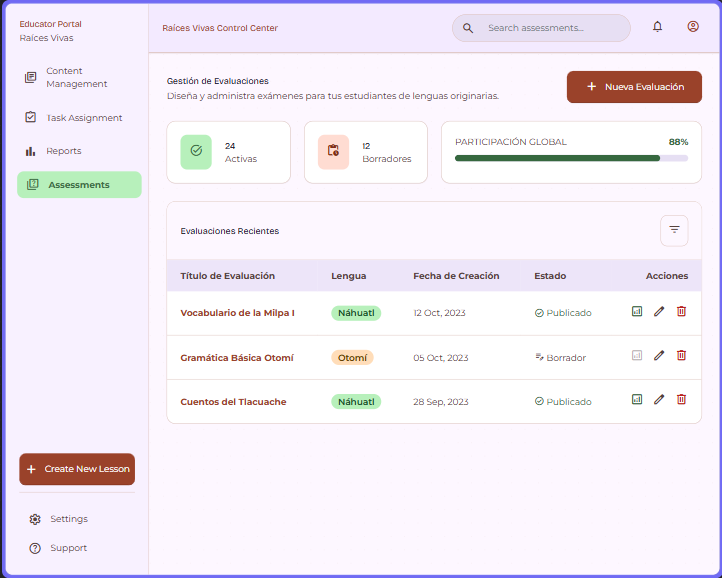
\includegraphics[height=4.8cm]{../img/Interfaces/Assessment_Creator__and__Manager.png}
    \par\vspace{0.4em}
    {\small\color{lighttext!70}Editor docente: Permite redactar reactivos, asignar puntajes y programar fechas de examen.}
\end{frame}

% Slide 30: Interfaz 17
\begin{frame}{Interfaz: Panel de Administración}
    \begin{tikzpicture}[remember picture,overlay]
        \node[anchor=north east, xshift=-0.3cm, yshift=-0.3cm] at (current page.north east) 
        {
\includegraphics[height=0.3cm]{../img/logos/CS_adjus.png}};
    \end{tikzpicture}
    \centering
    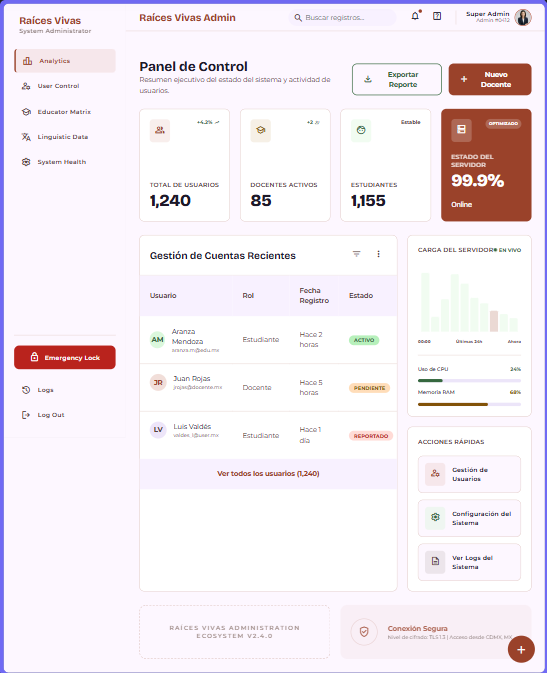
\includegraphics[height=4.8cm]{../img/Interfaces/General_Administration_Panel.png}
    \par\vspace{0.4em}
    {\small\color{lighttext!70}Módulo central del sistema: Configuración de roles, bitácoras e infraestructura.}
\end{frame}

% Slide 31: Interfaz 18
\begin{frame}{Interfaz: Gestión de Usuarios}
    \begin{tikzpicture}[remember picture,overlay]
        \node[anchor=north east, xshift=-0.3cm, yshift=-0.3cm] at (current page.north east) 
        {
\includegraphics[height=0.3cm]{../img/logos/CS_adjus.png}};
    \end{tikzpicture}
    \centering
    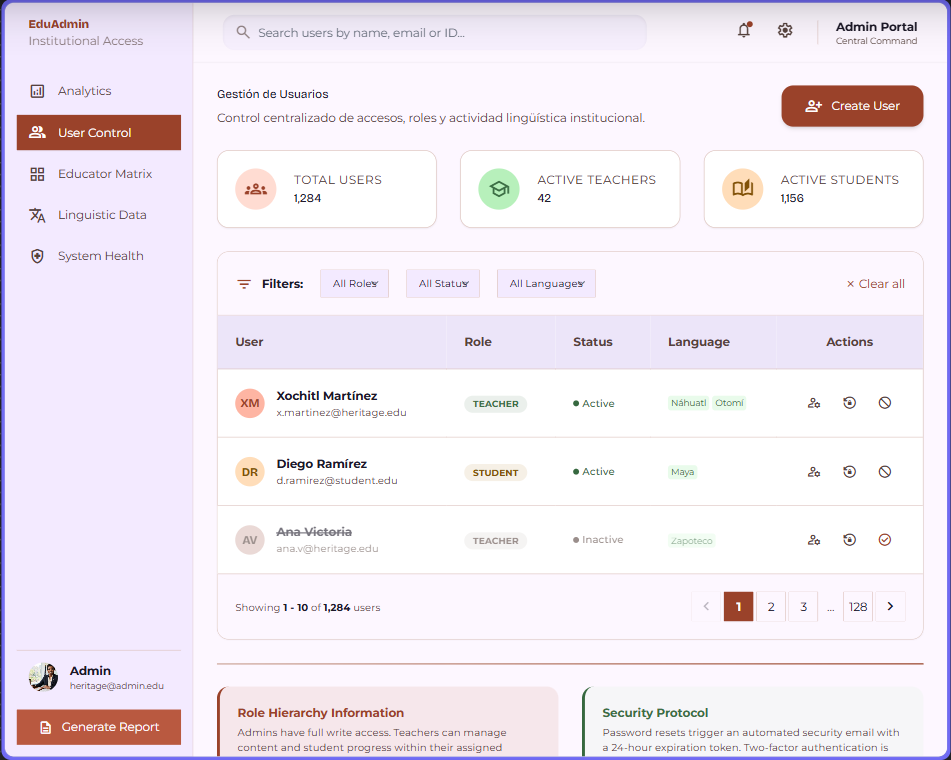
\includegraphics[height=4.8cm]{../img/Interfaces/User_Manager.png}
    \par\vspace{0.4em}
    {\small\color{lighttext!70}Administrador de cuentas: Altas, bajas, cambios y asignación de permisos especiales.}
\end{frame}

% Slide 32: Interfaz 19
\begin{frame}{Interfaz: Gestión de Recursos}
    \begin{tikzpicture}[remember picture,overlay]
        \node[anchor=north east, xshift=-0.3cm, yshift=-0.3cm] at (current page.north east) 
        {
\includegraphics[height=0.3cm]{../img/logos/CS_adjus.png}};
    \end{tikzpicture}
    \centering
    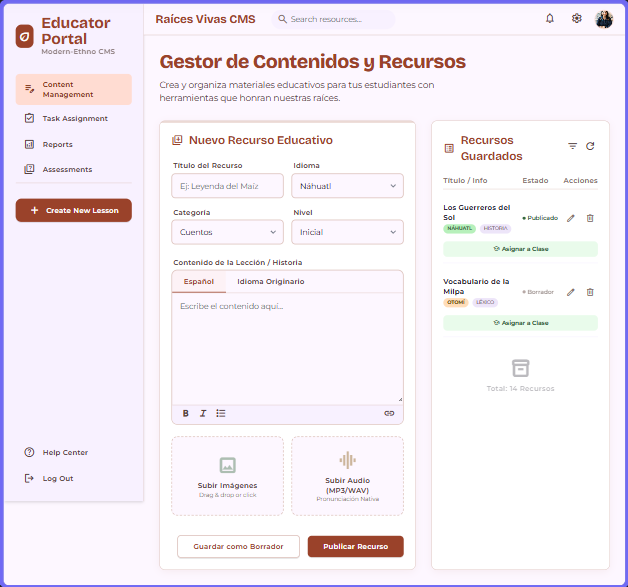
\includegraphics[height=4.8cm]{../img/Interfaces/Content__and__Resource_Manage.png}
    \par\vspace{0.4em}
    {\small\color{lighttext!70}Gestor de contenidos: Carga y administración de audios, textos e ilustraciones de cuentos.}
\end{frame}

% Slide 33: Interfaz 20
\begin{frame}{Interfaz: Configuración del Sistema}
    \begin{tikzpicture}[remember picture,overlay]
        \node[anchor=north east, xshift=-0.3cm, yshift=-0.3cm] at (current page.north east) 
        {
\includegraphics[height=0.3cm]{../img/logos/CS_adjus.png}};
    \end{tikzpicture}
    \centering
    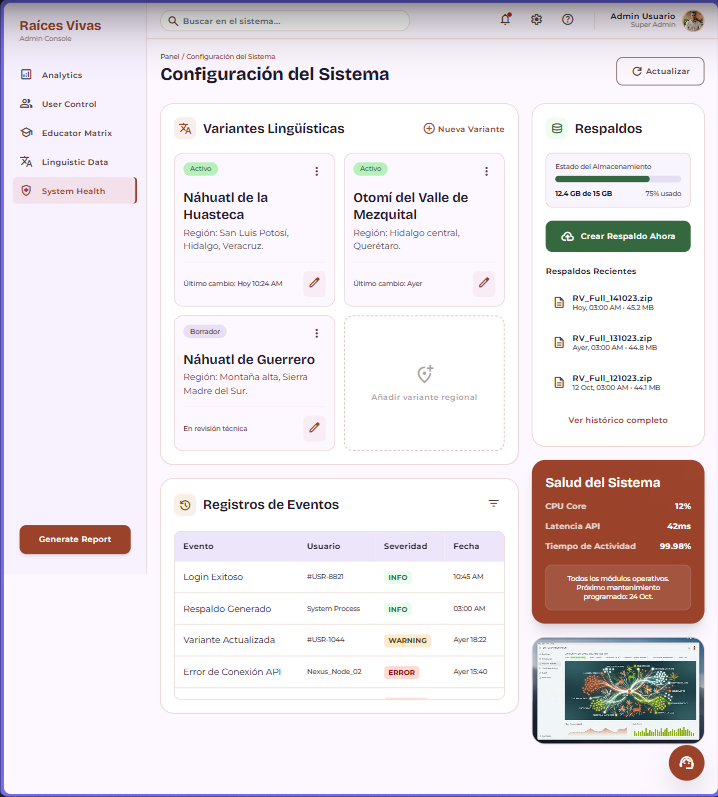
\includegraphics[height=4.8cm]{../img/Interfaces/System_Configuration.png}
    \par\vspace{0.4em}
    {\small\color{lighttext!70}Variables de entorno globales: Conexiones de base de datos, caché y tokens API.}
\end{frame}

% Slide 34: Parte 4 - Título
\begin{frame}[plain]
    \begin{tikzpicture}[remember picture,overlay]
        \node[anchor=north east, xshift=-0.3cm, yshift=-0.3cm] at (current page.north east) 
        {
\includegraphics[height=0.3cm]{../img/logos/CS_adjus.png}};
        \node[text=techblue, opacity=0.03, font=\bfseries, scale=35] at (current page.center) {4};
    \end{tikzpicture}
    \centering
    \vspace{2.2cm}
    {\huge\bfseries\color{techblue}PARTE 4: COSTOS,}\\[0.2em]
    {\huge\bfseries\color{techblue}SCRUM Y PLANIFICACIÓN}
\end{frame}

% Slide 35: Costos - Metodología de Estimación de Esfuerzo (NUEVA SLIDE)
\begin{frame}{Metodología de Estimación de Esfuerzo}
    \begin{tikzpicture}[remember picture,overlay]
        \node[anchor=north east, xshift=-0.3cm, yshift=-0.3cm] at (current page.north east) 
        {
\includegraphics[height=0.3cm]{../img/logos/CS_adjus.png}};
    \end{tikzpicture}
    \begin{columns}[onlytextwidth,c]
        \begin{column}{0.5\textwidth}
            \small
            \textbf{Técnica de Puntos de Historia (SP)}
            \begin{itemize}
                \item Estimación mediante la dinámica de \textbf{Planning Poker} para evaluar complejidad técnica.
                \item Backlog total estimado en \textbf{20 SP}.
                \item Factor de conversión: **1 SP $\approx$ 2 horas de desarrollo real**.
            \end{itemize}
        \end{column}
        
        \begin{column}{0.48\textwidth}
            \small
            \textbf{Horas Reales de Ingeniería}
            \begin{itemize}
                \item Esfuerzo neto de programación: \textbf{40.90 horas} totales.
                \item Tarifa por hora establecida: \textbf{\$350.00 MXN}.
                \item Se incluyó una holgura técnica de **15\%** ante contingencias o integración local.
            \end{itemize}
        \end{column}
    \end{columns}
\end{frame}

% Slide 36: Costos - Desglose Técnico por MR
\begin{frame}{Estimación de Costos por Solicitud (MR)}
    \begin{tikzpicture}[remember picture,overlay]
        \node[anchor=north east, xshift=-0.3cm, yshift=-0.3cm] at (current page.north east) 
        {
\includegraphics[height=0.3cm]{../img/logos/CS_adjus.png}};
    \end{tikzpicture}
    \centering\footnotesize
    \renewcommand{\arraystretch}{1.1}
    \begin{table}
        \color{lighttext}
        \begin{tabularx}{\textwidth}{Xcrr}
            \toprule
            \textbf{Solicitud de Modificación (MR)} & \textbf{Horas Base} & \textbf{Costo por Hora} & \textbf{Subtotal Neto} \\
            \midrule
            MR-001: Reconstitución Frontend (Crítica) & 16.00 h & \$350.00 MXN & \$5,600.00 MXN \\
            MR-002: Remoción de Bugs (Alta)          & 5.58 h  & \$350.00 MXN & \$1,953.00 MXN \\
            MR-003: Deuda Técnica y Linting (Baja)   & 1.32 h  & \$350.00 MXN & \$462.00 MXN \\
            MR-004: Filtros Lógicos CP007 (Aditiva)  & 8.00 h  & \$350.00 MXN & \$2,800.00 MXN \\
            MR-005: Persistencia CP008 (Aditiva)     & 10.00 h & \$350.00 MXN & \$3,500.00 MXN \\
            \midrule
            \textbf{Mano de Obra Directa (Neto)}     & \textbf{40.90 h} & --- & \textbf{\$14,315.00 MXN} \\
            \bottomrule
        \end{tabularx}
    \end{table}
\end{frame}

% Slide 37: Costos - Distribución y Costos Indirectos
\begin{frame}{Distribución de Presupuesto y Costos}
    \begin{tikzpicture}[remember picture,overlay]
        \node[anchor=north east, xshift=-0.3cm, yshift=-0.3cm] at (current page.north east) 
        {
\includegraphics[height=0.3cm]{../img/logos/CS_adjus.png}};
    \end{tikzpicture}
    \begin{columns}[onlytextwidth,c]
        \begin{column}{0.48\textwidth}
            \footnotesize
            \textbf{Desglose de Costos del Proyecto}
            \begin{itemize}
                \item \textbf{Costo Directo (Ingeniería):} \$14,315.00 MXN (40.90 h).
                \item \textbf{Instancia SonarQube:} \$0.00 MXN (Mitigado mediante uso de Community Edition local).
                \item \textbf{Amortización e Infraestructura Sandbox:} \$350.00 MXN (Consumo eléctrico y desgaste de hardware).
            \end{itemize}
            \vspace{0.5em}
            \centering
            \begin{tikzpicture}
                \node[draw=accentgreen, fill=cardbg, thick, rounded corners=4pt, inner sep=6pt, text width=5.0cm, align=center] {
                    \color{lighttext}\scriptsize Costo Total Consolidado:\\[0.15em]
                    \color{accentgreen}\bfseries\normalsize \$14,665.00 MXN
                };
            \end{tikzpicture}
        \end{column}
        
        \begin{column}{0.48\textwidth}
            \centering
            % Diagrama de barras en TikZ
            \begin{tikzpicture}[
                scale=1.1, transform shape,
                bar/.style={draw=techblue, fill=techblue!30, thick},
                label/.style={font=\tiny, text=lighttext, anchor=east}
            ]
                \fill[cardbg] (0,0) rectangle (4,2.5);
                
                % MR-001
                \node[label] at (1.1, 2.1) {MR-001};
                \draw[bar] (1.2, 2.0) rectangle (1.2 + 2.4, 2.2);
                
                % MR-005
                \node[label] at (1.1, 1.7) {MR-005};
                \draw[bar] (1.2, 1.6) rectangle (1.2 + 1.5, 1.8);
                
                % MR-004
                \node[label] at (1.1, 1.3) {MR-004};
                \draw[bar] (1.2, 1.2) rectangle (1.2 + 1.2, 1.4);
                
                % MR-002
                \node[label] at (1.1, 0.9) {MR-002};
                \draw[bar] (1.2, 0.8) rectangle (1.2 + 0.8, 1.0);
                
                % MR-003
                \node[label] at (1.1, 0.5) {MR-003};
                \draw[bar] (1.2, 0.4) rectangle (1.2 + 0.2, 0.6);
                
                \draw[->, thick, lighttext] (1.1, 0.2) -- (1.1, 2.4);
                \draw[->, thick, lighttext] (1.1, 0.2) -- (3.8, 0.2);
            \end{tikzpicture}
        \end{column}
    \end{columns}
\end{frame}

% Slide 38: Parte 4 - Estructura Scrum Team
\begin{frame}{Estructura SCRUM y Ceremonias}
    \begin{tikzpicture}[remember picture,overlay]
        \node[anchor=north east, xshift=-0.3cm, yshift=-0.3cm] at (current page.north east) 
        {
\includegraphics[height=0.3cm]{../img/logos/CS_adjus.png}};
    \end{tikzpicture}
    \begin{columns}[onlytextwidth,c]
        \begin{column}{0.48\textwidth}
            \textbf{Estructura del Scrum Team}
            \begin{itemize}
                \item \textbf{Product Owner}: Mtra. Alicia Ortiz Montes (valida incrementos y define prioridades).
                \item \textbf{Scrum Master}: Sánchez Romero José Enrique (remueve bloqueos, gestiona sandbox y flujos).
                \item \textbf{Development Team}: Brandon Chavarría, Emmanuel Islas, Kenneth Morán.
            \end{itemize}
        \end{column}
        
        \begin{column}{0.48\textwidth}
            \textbf{Ceremonias Ágiles (Sprints de 2 Semanas)}
            \begin{itemize}
                \item \textbf{Sprint Planning}: Primer lunes (desglose de tareas y estimación de SP).
                \item \textbf{Daily Standup}: Mar a Vie, 15 min (sincronización rápida y alertas).
                \item \textbf{Review \& Retro}: Último viernes (demostración en vivo ante PO y retrospectiva).
            \end{itemize}
        \end{column}
    \end{columns}
\end{frame}

% Slide 39: Parte 4 - Cronograma de Sprints
\begin{frame}{Planificación de Sprints (2 Semanas)}
    \begin{tikzpicture}[remember picture,overlay]
        \node[anchor=north east, xshift=-0.3cm, yshift=-0.3cm] at (current page.north east) 
        {
\includegraphics[height=0.3cm]{../img/logos/CS_adjus.png}};
    \end{tikzpicture}
    \textbf{Sprint 1: Infraestructura y Datos (Semanas 1-2)}
    \begin{itemize}
        \item \textbf{Meta:} Estabilizar el entorno e iniciar la persistencia.
        \item \textbf{Backlog:} US-001 (8 SP) + US-002 (5 SP) = \textbf{13 SP}.
        \item \textbf{Trabajo:} Levantar React-Vite, migrar tabla \path{progress} y programar controlador de persistencia.
    \end{itemize}
    \vspace{0.4em}
    \textbf{Sprint 2: Lógica y Calidad (Semanas 3-4)}
    \begin{itemize}
        \item \textbf{Meta:} Filtros dinámicos y remediación estática.
        \item \textbf{Backlog:} US-003 (3 SP) + US-004 (3 SP) + US-005 (1 SP) = \textbf{7 SP}.
        \item \textbf{Trabajo:} Programar filtros de búsqueda, configurar linters y remover bugs SonarQube.
    \end{itemize}
\end{frame}

% Slide 40: Conclusión de la Propuesta de Mantenimiento
\begin{frame}{Conclusión y Resultados}
    \begin{tikzpicture}[remember picture,overlay]
        \node[anchor=north east, xshift=-0.3cm, yshift=-0.3cm] at (current page.north east) 
        {
\includegraphics[height=0.3cm]{../img/logos/CS_adjus.png}};
    \end{tikzpicture}
    \textbf{Beneficios del Plan Ejecutado}
    \begin{itemize}
        \item \textbf{Recuperación Arquitectónica}: Reconstitución del frontend React enlazado a Laravel vía Inertia.js.
        \item \textbf{Estabilidad Operativa}: Persistencia real del progreso infantil en base de datos PostgreSQL en producción.
        \item \textbf{Calidad Certificada}: Disminución a cero de bugs de fiabilidad detectados en análisis estático.
        \item \textbf{Sostenibilidad}: Mantenibilidad clasificada en categoría A, facilitando la futura adición de juegos didácticos y cuentos interactivos.
    \end{itemize}
\end{frame}

% Slide 41: Próximos Pasos del Proyecto (NUEVA SLIDE)
\begin{frame}{Siguientes Pasos del Proyecto}
    \begin{tikzpicture}[remember picture,overlay]
        \node[anchor=north east, xshift=-0.3cm, yshift=-0.3cm] at (current page.north east) 
        {
\includegraphics[height=0.3cm]{../img/logos/CS_adjus.png}};
    \end{tikzpicture}
    \textbf{Acciones Inminentes Planificadas}
    \begin{itemize}
        \item \textbf{Programación y Despliegue}: Iniciar de forma sistemática la programación y despliegue del resto de los módulos funcionales del sistema Yoliztli.
        \item \textbf{Pruebas de Integración y Regresión}: Realizar las pruebas correspondientes para cada uno de los módulos desarrollados, garantizando su acoplamiento sin regresiones de software.
        \item \textbf{Aseguramiento de Calidad}: Mantener el monitoreo continuo a través de SonarQube para evitar la inyección de nueva deuda técnica en producción.
    \end{itemize}
\end{frame}

% Slide 42: Cierre / Agradecimientos (GRACIAS simple y cita)
\begin{frame}[plain]
    \begin{tikzpicture}[remember picture,overlay]
        % Marco decorativo perimetral delgado en cian para el cierre
        \draw[accentcyan, line width=2pt] 
        ([xshift=0.2cm, yshift=-0.2cm]current page.north west) rectangle 
        ([xshift=-0.2cm, yshift=0.2cm]current page.south east);
        % Logo de la consultora en la esquina superior derecha
        \node[anchor=north east, xshift=-0.4cm, yshift=-0.4cm] at (current page.north east) 
        {
\includegraphics[height=0.4cm]{../img/logos/CS_adjus.png}};
    \end{tikzpicture}
    \centering
    \vspace{1.5cm}
    {\Huge\bfseries\color{accentcyan}GRACIAS}\\[1.5em]
    
    \begin{minipage}{0.85\textwidth}
        \centering
        \itshape\color{white}\Large
        ``Los buenos programadores escriben código que los humanos pueden entender.''
        \par\vspace{1.0em}
        \hfill\upshape\color{techblue}\large --- Martin Fowler
    \end{minipage}
\end{frame}

\end{document}
